\documentclass[a4paper,12pt]{article}
\usepackage{pdfpages}
\usepackage[T1]{fontenc}
\usepackage[utf8]{inputenc}
\usepackage{floatflt}
\usepackage{float}
\usepackage[font=small,labelfont=bf]{caption}
\usepackage{graphicx}
\graphicspath{{figures/}}
\usepackage[english]{babel}
\usepackage{underlin}
\usepackage{footnote}
\usepackage{wrapfig}
\usepackage{url}
\setcounter{secnumdepth}{4} 
\setcounter{tocdepth}{4} 
\pagestyle{underline}
\newcommand{\superscript}[1]{\ensuremath{^{\textrm{#1}}}}
\newcommand{\subscript}[1]{\ensuremath{_{\textrm{#1}}}}
\setlength{\parindent}{0pt}
	
%----------------------------------------------------------------------------
%Front page
%----------------------------------------------------------------------------
\begin{document}
\begin{titlepage}
	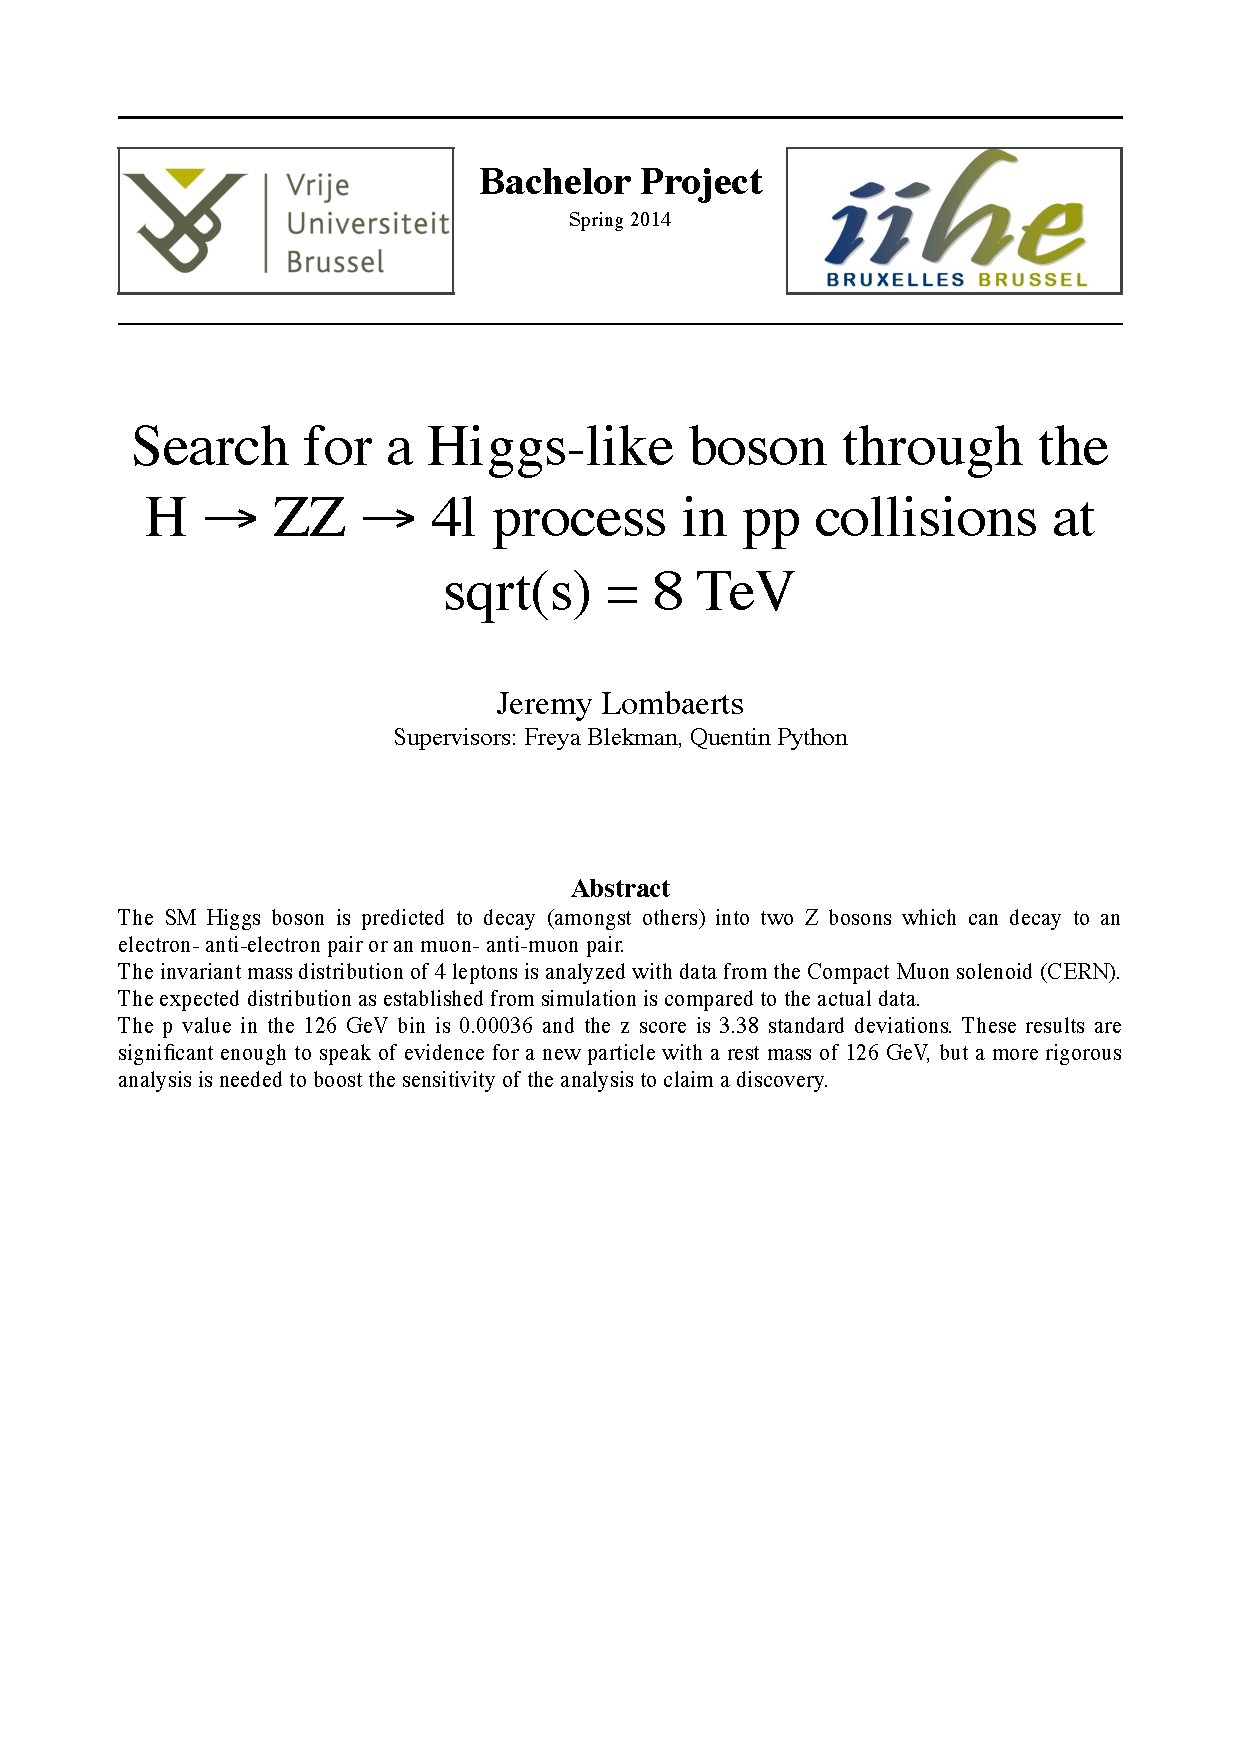
\includepdf{titelpage.pdf}
\end{titlepage}
\newpage




%----------------------------------------------------------------------------
%Contents
%----------------------------------------------------------------------------
\newpage 
\tableofcontents
\newpage




%----------------------------------------------------------------------------
%Introduction
%----------------------------------------------------------------------------
\section{Introduction}
\subsection{The Standard Model of Physics}
\begin{wrapfigure}{r}{.6\textwidth}
	\centering
	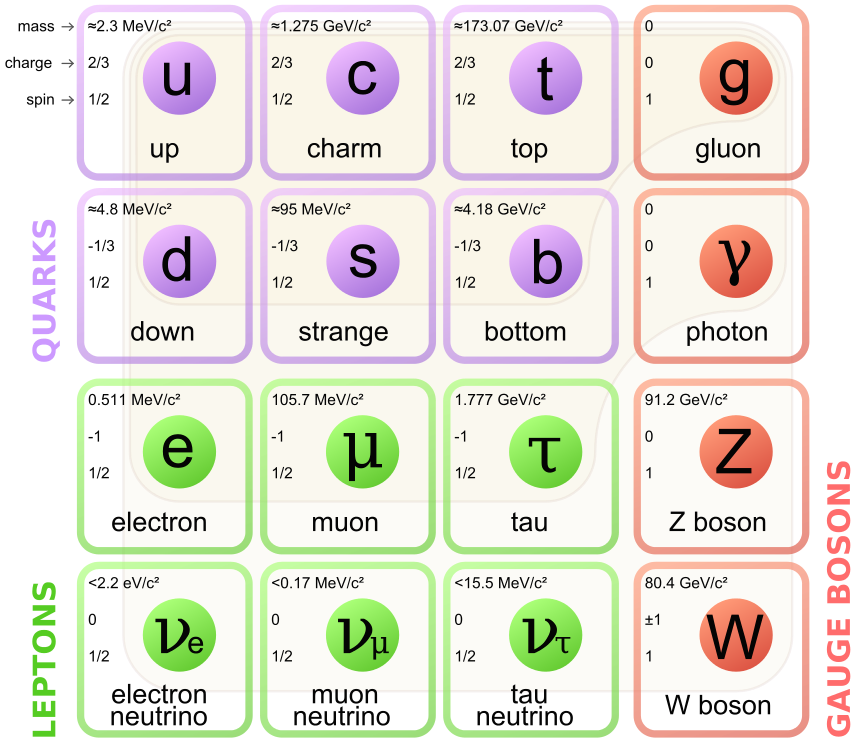
\includegraphics[width=0.6\textwidth]{sm1.png}
	\caption{\emph{The SM fundamental particles: Quarks, leptons and gauge bosons}}
	\label{fig:sm1}
\end{wrapfigure}
The Standard Model (SM) of physics \cite{sm} is a theory that describes the dynamic of all known subatomic particles. It is based on the insight that everything in nature is made up of combinations of a few subatomic particles (fig. \ref{fig:sm1}). These particles interact with each other through the four fundamental forces: the gravitational force, the electromagnetic force, the weak nuclear force and the strong nuclear force. The SM only describes the  electromagnetic, weak and strong nuclear forces. Gravity has not (yet) been incorporated in the SM. Though the SM has been experimentally verified numerous times and has made correct predictions in the past, it is not a complete theory because it fails to answer some fundamental questions such as the dark matter problem and the lack of anti-matter in the observable universe, amongst others.




\subsubsection{Fermions and bosons}
Fermions are particles with half-integer spin, therefore governed by Fermi-Dirac statistics. They obey Pauli's exclusion principle. All quarks and leptons are fermions.\\ 
Bosons are particles with integer spin, therefore governed by Bose-Einstein statistics. All discovered fundamental bosons are force carriers. These fundamental, force carrying particles are referred to as "gauge bosons". The photon ($\gamma$) mediates the electromagnetic force, the gluons (g) mediate the strong nuclear force and the W and Z bosons (W\superscript{+}, W\superscript{-}, Z\superscript{0}) mediate the weak nuclear force. The Higgs boson (H\superscript{0}) could be the first fundamental boson to be discovered that does not mediate one of the fundamental forces.




\subsubsection{The Brout-Englert-Higgs mechanism}
In the SM photons are massless, but the W and Z bosons are massive. Englert and Brout \cite{paper1}; Higgs \cite{paper2}; Guralnik, Hagen and Kibble \cite{paper3} proposed a modification to the SM by introducing a symmetry breaking mechanism (BEH [Brout-Englert-Higgs] mechanism) capable of attributing mass to the massive gauge bosons. Elementary fermions would get their mass through a Yukawa interaction. 
\\Experimental verification of the BEH model could be done by observing a new fundamental particle: the scalar (spin = 0) Higgs boson. In the BEH model the mass of the Higgs boson is a free parameter. This complicates the search for such a boson. The properties of the Higgs boson are strongly correlated to its mass. Being able to experimentally detect a Higgs boson would give credence to the BEH model and again confirm the self consistency of the SM.




\subsubsection{Properties of the Higgs boson}
\begin{wrapfigure}{r}{0.38\textwidth}
	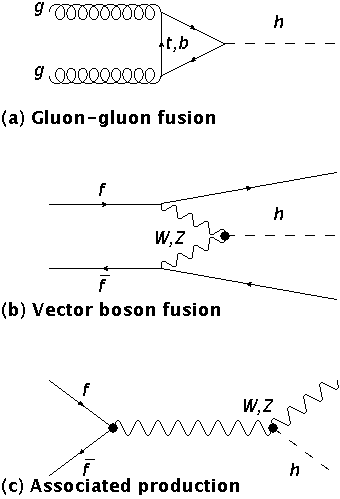
\includegraphics[width=0.38\textwidth]{higgsProduction.png}
	\caption{\emph{Higgs boson production mechanisms}}
	\label{fig:higgsProduction1}
\end{wrapfigure}
\textbf{Producing the Higgs boson}
\newline
To be able to identify Higgs bosons, it is essential to understand how such bosons can be created \cite{two}. 
\\The most efficient way to produce Higgs bosons at the LHC is gluon-gluon fusion (GGF)(fig. \ref{fig:higgsProduction1}a): two gluons from colliding protons fuse together and from a Higgs boson through an intermediate virtual quark loop. Because the coupling to the Higgs boson is proportional to the mass of the particles, this process is more likely to involve the heaviest quarks. In practice it is enough to consider the contribution of the top and bottom quark. 
\\A second mechanism capable of producing Higgs bosons is vector boson fusion (VBF)(fig. \ref{fig:higgsProduction1}b). When two, not necessarily the same (anti-) fermions collide, they exchange a virtual W or Z boson which radiates a Higgs boson.
\\The third option is associated production (fig. \ref{fig:higgsProduction1}c). An elementary fermion colliding with its anti particle can produce a W or Z boson. This W or Z boson can emit a Higgs boson if enough energy is available.
\newline
\textbf{Decay modes of the Higgs boson \cite{branching}}
\newline
If a heavy particle can decay to a lighter particle, it will do so. The half life time of heavy particles depends on a variety of factors, including the mass difference between the concerned particles, the strength of the interaction between the various particles,... Most of these factors are fixed within the SM. For a Higgs boson with a mass around $126$ GeV the SM predicts a mean half life time of $1.56\times10^{-22}$ s.
\\The Higgs boson interacts with all massive particles, giving it a wide array of decay possibilities (fig. \ref{fig:higgsdecay1}). The cross sections and branching ratios for each of these modes depend on the Higgs mass (fig. \ref{fig:higgsdecay1}). 
\\This analysis focusses primarily on the H $\rightarrow$ ZZ $\rightarrow$ 4l process. This is not the most probable decay mode, but the four leptons usually leave very clear tracks in the detector and the background is rather easy to evaluate, making this the easiest process to analyze.
\begin{figure}[!hb]
	\centering
 	\begin{minipage}[cb]{0.49\textwidth}
   	\centering
		\begin{tabular}{l  l}
			\textbf{Decay mode}												& \textbf{BR (\%)}\\
		    \hline
			H $\rightarrow$ b$\bar{b}$										& $5.61\times10^{-01}\ ^{+3.3}_{-3.4}$\\
			H $\rightarrow$ $\tau$\superscript{+}$\tau$\superscript{-}		& $6.15\times10^{-02}\ ^{+5.6}_{-5.6}$\\
			H $\rightarrow$ $\mu$\superscript{+}$\mu$\superscript{-}		& $2.14\times10^{-04}\ ^{+5.9}_{-5.8}$\\
			H $\rightarrow$ c$\bar{c}$										& $2.83\times10^{-02}\ ^{+12.2}_{-12.2}$\\
			\\
			H $\rightarrow$ gg												& $8.48\times10^{-02}\ ^{+10.1}_{-9.9}$\\
			H $\rightarrow$ $\gamma\gamma$									& $2.28\times10^{-03}\ ^{+4.9}_{-4.8}$\\
			H $\rightarrow$ Z$\gamma$										& $1.62\times10^{-03}\ ^{+8.9}_{-8.8}$\\
			H $\rightarrow$ WW												& $2.31\times10^{-01}\ ^{+4.41}_{-4.1}$\\
			H $\rightarrow$ ZZ												& $2.89\times10^{-02}\ ^{+4.12}_{-4.0}$\\
		\end{tabular}
 	\end{minipage}
 	\begin{minipage}[cb]{0.49\textwidth}
   	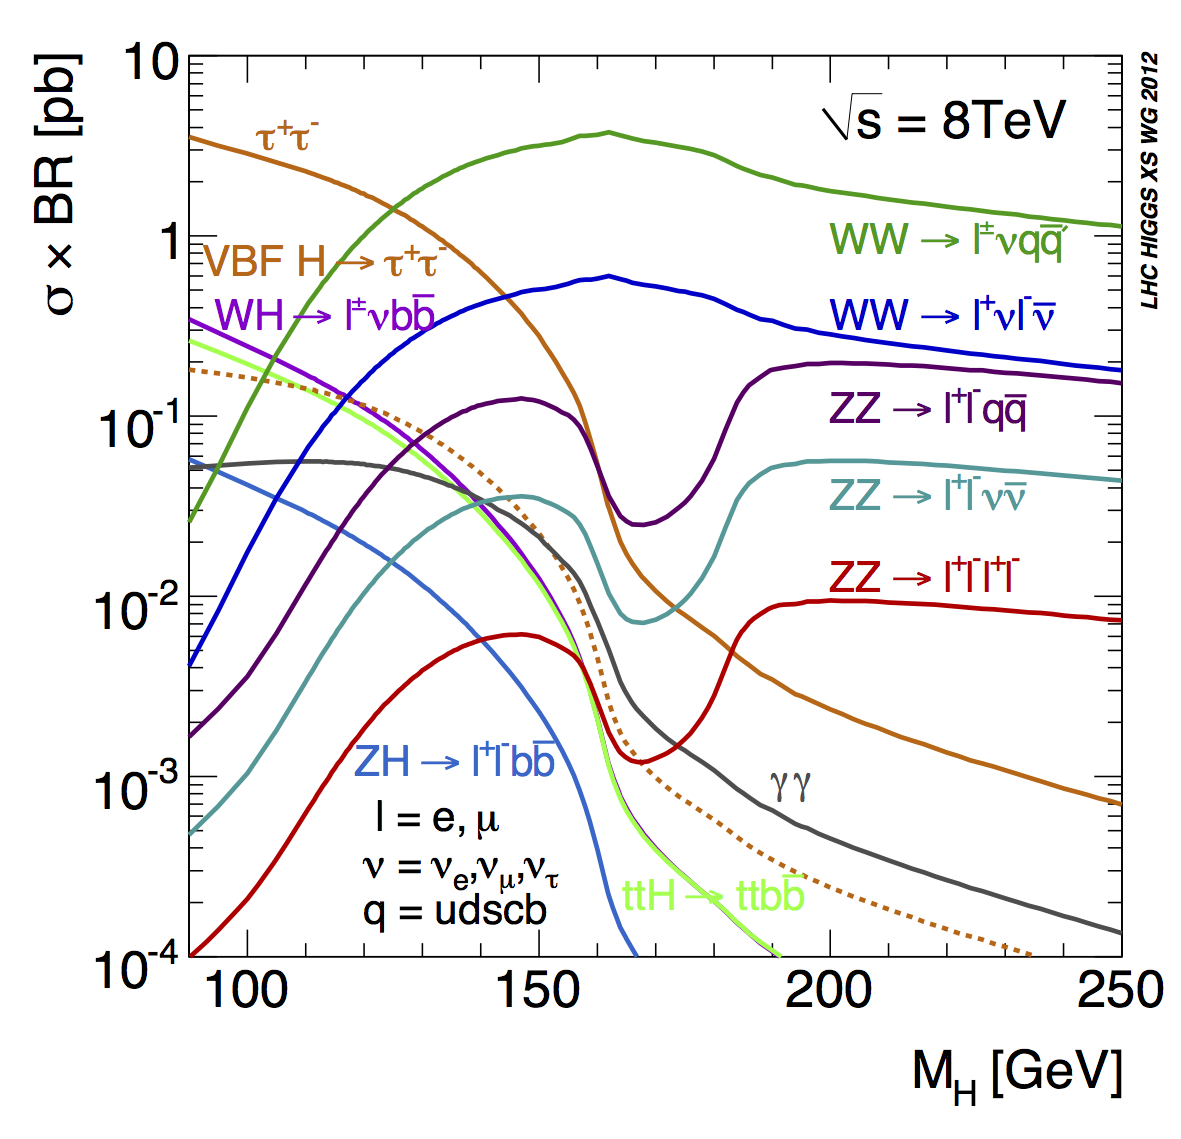
\includegraphics[width=0.85\textwidth]{higgsDecayCrossSections.png}
 	\end{minipage}
 	\caption{\emph{(Left) The branching ratios for the various decay modes of the Higgs boson with $m_H=126\ GeV$are listed with their theoretical uncertainty.\\(Right) The total cross section for the various Higgs end products depends on the Higgs mass. The uncertainties are pictured as bands around the mean value.}}
	\label{fig:higgsdecay1}
\end{figure}
\newline
\newline
\textbf{Mass of the Higgs boson}
\newline
The BEH model does not specify the mass of the Higgs boson, which makes it more difficult to find it. Previous searches for the Higgs boson at the LHC have excluded the mass region below 114.4 GeV and experiments at Fermilab's Tevatron particle accelerator have already excluded a narrow region around 160 GeV. The Tevatron data does show an excess of events in the mass region around 126 GeV, hinting at a possible new particle \cite{cern}.




\subsection{Particle physics at CERN}
\subsubsection{The Large Hadron Collider}
The Large Hadron Collider (LHC) is a circular particle accelerator. It is designed to accelerate and collide protons and heavy lead ions. 
\\The LHC has a circumference of 27 km and lies around 175 m deep, making it the biggest and most powerful accelerator to date. It collides proton-proton beams at an energy of $\sqrt{s} = 8$ TeV (2012) with an integrated luminosity $\mathcal{L}$ of 19.6 fb\superscript{-1} \cite{one}. The various LHC experiments generate tens of petabytes of data every year. Storing and analyzing data is done by grid computing.
\\There are four main interaction points at the LHC. Detectors are installed at every interaction point to analyze the collisions. The main detectors are the Compact Muon Solenoid (CMS), A Toroidal LHC Apparatus (ATLAS), LHC-Beauty (LHCb) and A Large Ion Collider Experiment (ALICE). This analysis uses data recorded by CMS. ATLAS has goals very similar to CMS while LHCb and ALICE have more specific goals.




\subsubsection{The CMS experiment}
CMS \cite{cms} is designed to detect high-energy subatomic particles generated through proton-proton and heavy-ion collisions. The main feature is a 3.8T uniform magnetic field, generated along the beam axis by a superconducting solenoid. The detector consists of a layered cylinder, the barrel, and endcap disks (fig. \ref{fig:cms1}). 
\newline
\newline
\textbf{The interaction point}
\newline
The interaction point is where the particle beams collide. Magnets at both ends of the detector focus the beams into the interaction point. When colliding, every beam has a diameter of $17\ \mu$m. The crossing angle is $285\ \mu$rad. At full luminosity each beam contains 2808 bunches of $1.15\times10^{11}$ protons. The time interval between two bunches is currently 50 ns but will be decreased to 25 ns.
\newline
\newline
\textbf{Tracker}
\newline
Close to the interaction point are silicon trackers and strips capable of detecting electrons, high-energy muons and charged hadrons. The tracker is used to determine the path of the particles generated in collisions. The measured path is used to get the particle's momentum.
\\Charged particles moving in a magnetic field follow a curved path. The curvature is related to the momentum of the particle: the more the track is curved, the lesser momentum the particle has. By measuring the position of the particle at various key points the particle path and momentum are reconstructed. 
\newline
\newline
\textbf{Electromagnetic calorimeter}
\newline
The electromagnetic calorimeter (ECAL) is used to detect and measure the energies of electrons and photons. It consists of lead-tungstate (PbWO\subscript{4}) crystals. These are very heavy (heavier than steel) crystals, yet are completely transparent. Electrons and photons passing through these crystals cause scintillation inside the crystals proportionate to the particles energy. Measuring the scintillation light provides information about the energy of the particles stopped by the crystals.
\newline
\newline
\textbf{Hadronic calorimeter}
\newline
The energy of hadrons is being measured in the barrel hadron calorimeter (HCAL) and the hadronic forward calorimeter (HF). 
\\The HCAL is made of dense (steel/brass), layered material. In-between the dense layers are plastic scintillators.
\\The HF is capable of measuring pseudorapidities in the range $3.0 < \eta < 5.0$. Its functioning is slightly different from the HCAL, but both serve the same purpose. The HF is also used to mesure CMS's instant luminosity. 
\begin{figure}[!hb]
	\centering
	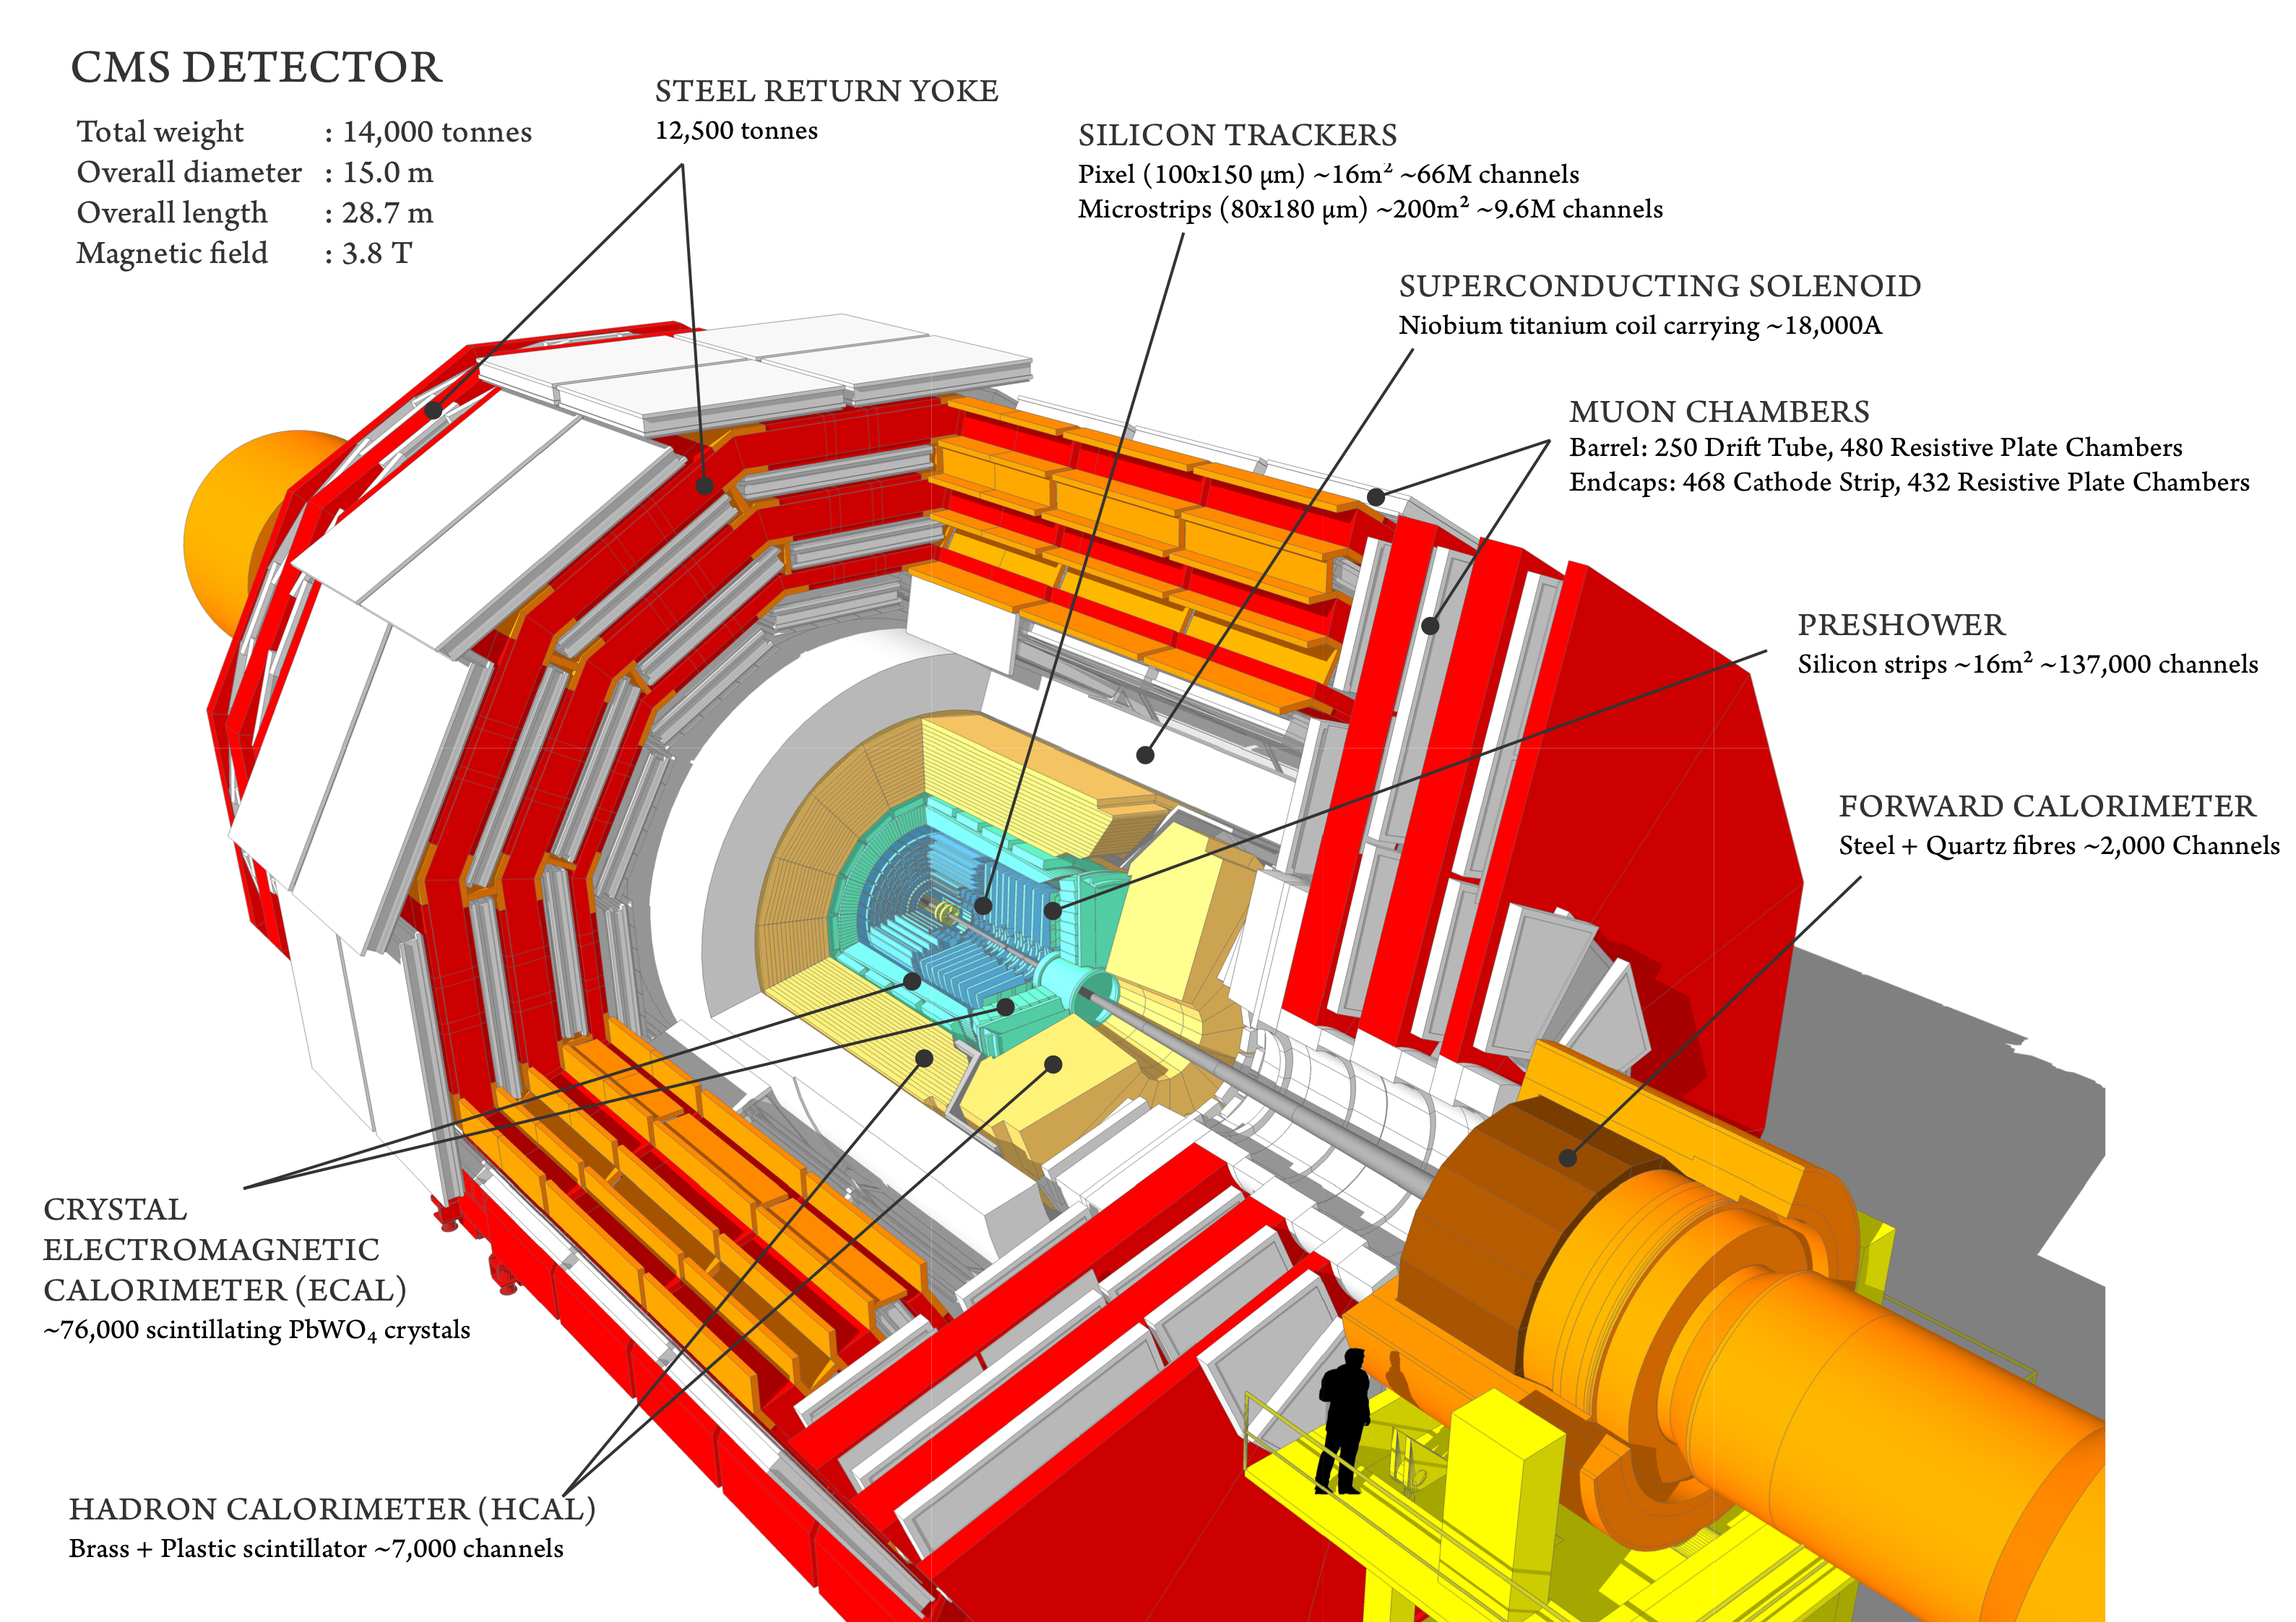
\includegraphics[width=0.9\textwidth]{cms.png}
	\caption{\emph{The CMS detector and its main components}}
	\label{fig:cms1}
\end{figure}\\
\textbf{Solenoid}
\newline
The second to last layer of the detector is the superconducting solenoid generating an uniform 3.8 T magnetic field. The solenoid also provides structural strength to the whole detector structure. it must be strong enough to resist its own magnetic field while carrying part of the detector. 
\newline
\newline
\textbf{Muon detectors and iron return yoke}
\newline
One of CMS's main tasks is the detection of muons, predicted to be generated in the decay of various hypothetical particles.
\\Muons have a mass of 105.6 MeV and are about 200 times heavier than electrons. Their mean lifetime is 2.2 $\mu$s (special relativity, mean lifetime to be measured in the muon's frame of reference). 
\\When moving through matter, muons do not decelerate as sharply as electrons do due to their inertia. This limits the bremsstrahlung emitted by muons. Bremsstrahlung being the prominent mechanism through which electrons and muons lose kinetic energy in matter, muons have a higher penetrating ability than electrons. Therefore muons are not likely to be stopped by the ECAL or HCAL. Thus the only particles likely to produce signals on the outer edges of the detector are muons. The muon detectors used in the barrel differ from those in the endcap disks. The drift tubes used in the barrel allow precise trajectory measurements in the central barrel region. The cathode strip chambers are used in the endcap disks. In both barrel and endcap disks resistive plate chambers produce fast signals when muons pass through them.




\subsubsection{Coordinate conventions}
The right handed Cartesian (xyz) coordinate system in CMS has been chosen to allow for easy conversions to other coordinate systems. The x-axis lies horizontal in the transverse plane. The y-axis points upwards. The z-axis lies along the beam axis so that the Cartesian coordinate system is right handed. The relativistic nature of the experiment suggests the use of 4-vectors \cite{relativity}. The fourth coordinate is the time.
\\CMS uses HEP (High Energy Physics) coordinates (E, $\phi$, P\subscript{T}, $\eta$) where E is the particle's energy and $\phi$ is the polar angle in the transverse plane. P\subscript{T} is the transverse momentum. The transverse momentum is the vector sum of the momentum along the x-axis and along the y-axis, with the z-axis lying along the beam axis. 
\begin{eqnarray}
	P_{T} &=& \sqrt{P{_X}^2 + P{_Y}^2}
\end{eqnarray}
$\eta$ is the pseudorapidity. The pseudorapidity is a measure for the angle the particle makes with the beam axis. The pseudorapidity is defined as
\begin{eqnarray}
	\eta &=& -ln \left ( tan \left ( \frac{\theta}{2} \right ) \right )
\end{eqnarray}
$\eta$ increases from 0 to $+\infty$ as the angle with the beam axis decreases from $\frac{\pi}{2}$ rad to $0$ rad.
\\CMS provides full azimuthal coverage for the detection of particles, but is not capable of detecting particles over the whole pseudorapidity range due to the beam pipe obstructing the view on the one hand and due to the junction between barrel and endcap not being perfect for various detectors parts on the other hand (fig. \ref{fig:etacms1}). Figure \ref{fig:eta1} (left) shows a distinct drop in electron events around $\eta$ = 1.5, corresponding to the junction between the barrel ECAL and endcap ECAL. Both plots show abrupt cuts around $\eta$ = 2.4. This is due to the tracker not being able to measure $\eta$ > 2.4 (fig. \ref{fig:etacms1}), and events without a tracker signal are not selected.
\enlargethispage{2\baselineskip}
\begin{figure}[!h]
	\centering
	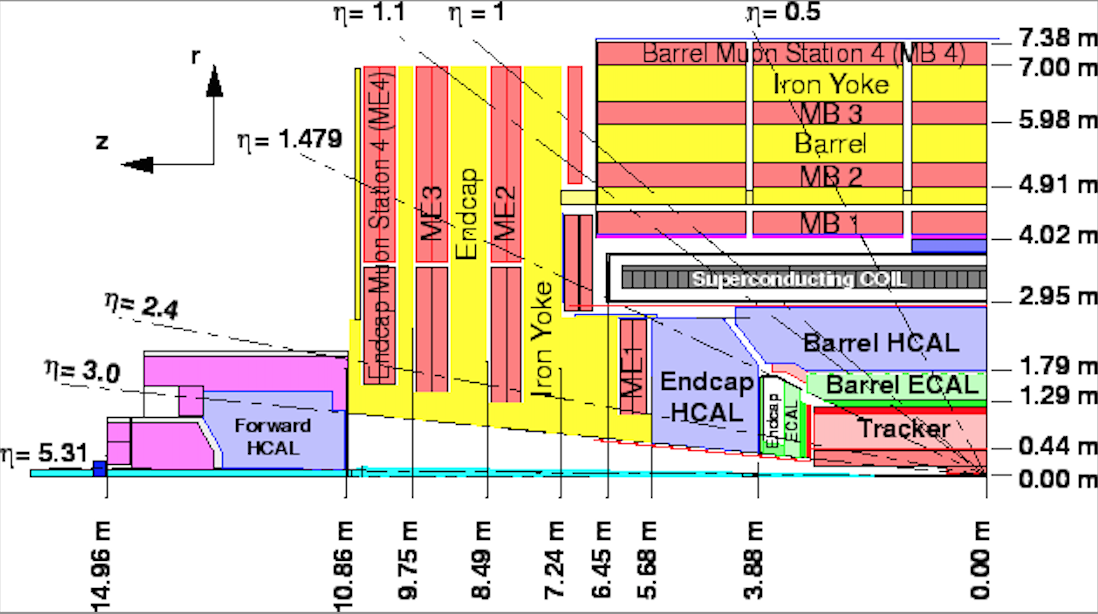
\includegraphics[width=.6\textwidth]{etaCms.png}
	\caption{\emph{The pseudorapidity in CMS: Imperfection in the detector create blind spots.}}
	\label{fig:etacms1}
\end{figure}
\begin{figure}[!h]
	\begin{minipage}[b]{.5\linewidth}
 		\centering
 		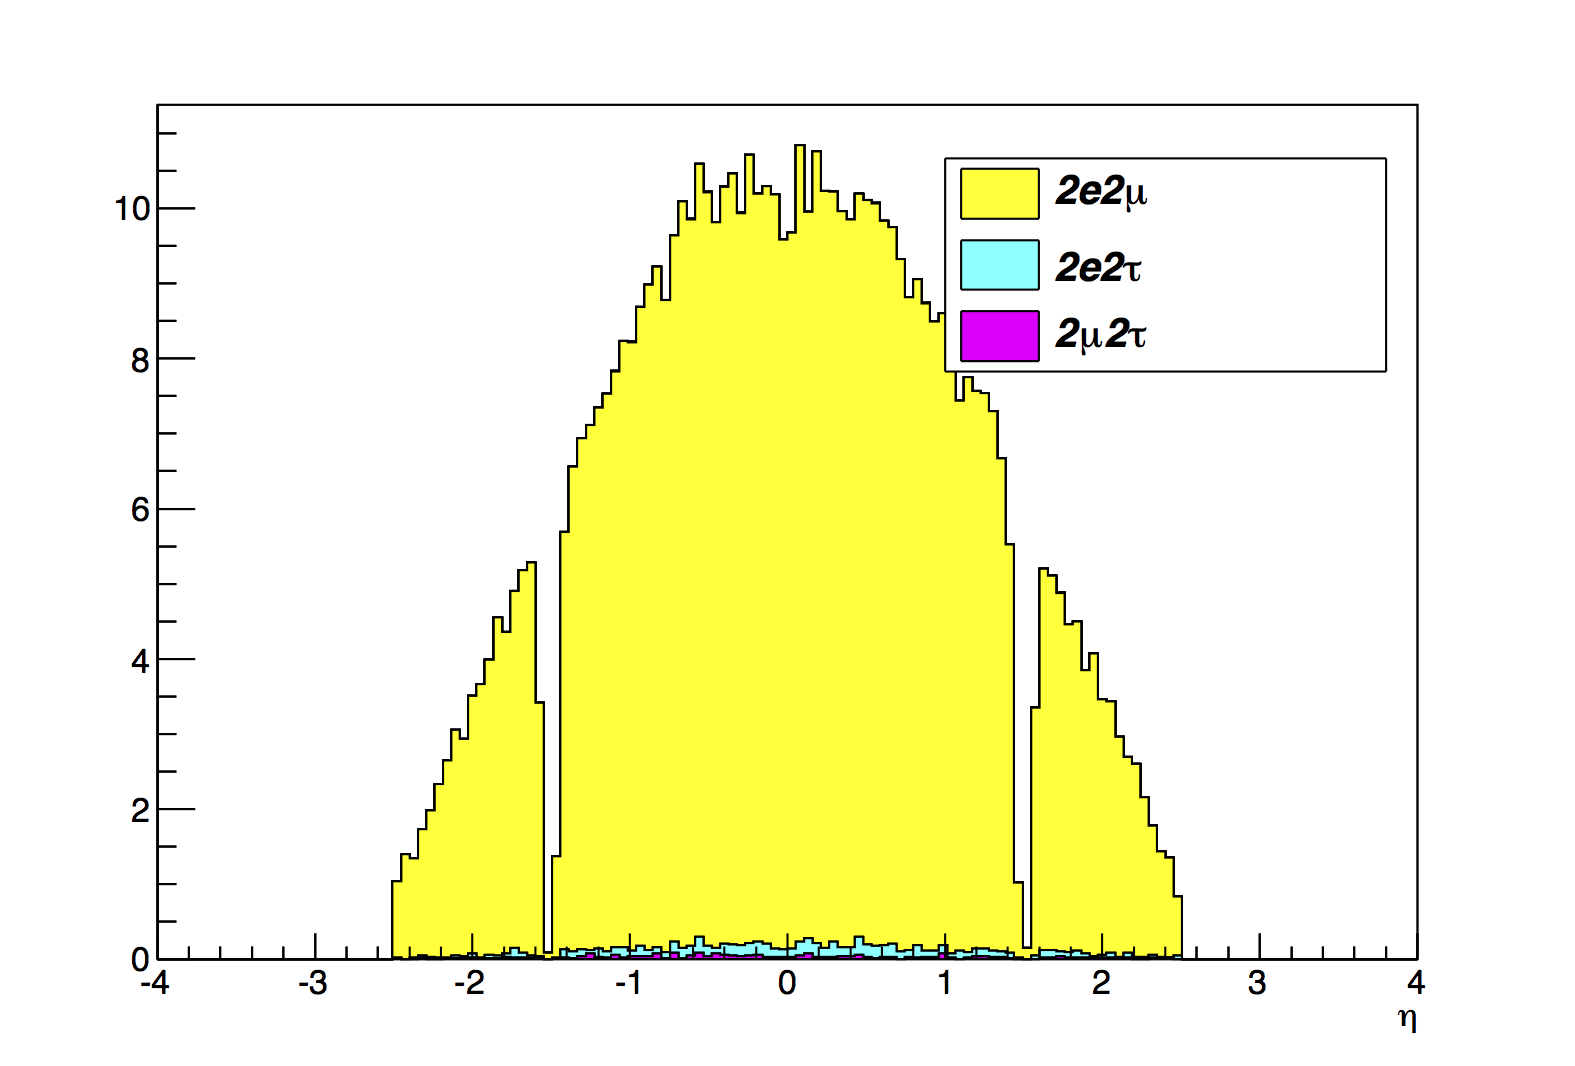
\includegraphics[scale=.3]{etaelectrons.png}
	\end{minipage}
	\begin{minipage}[b]{.5\linewidth}
 	  	\centering
 	  	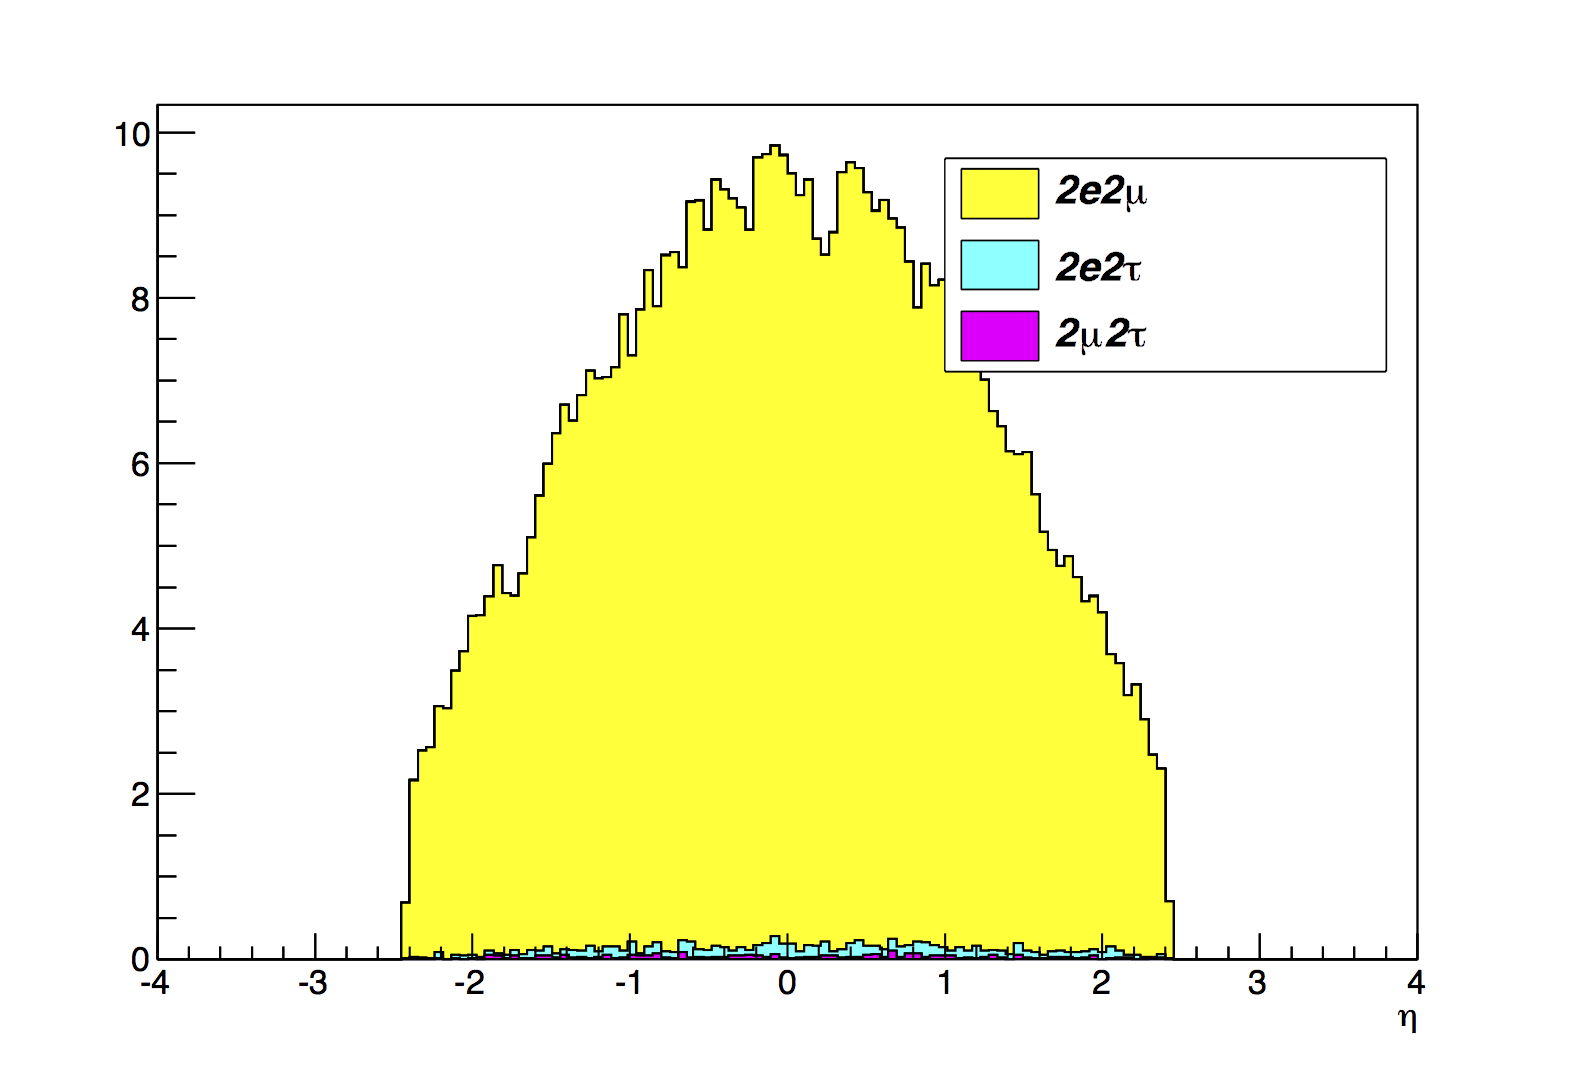
\includegraphics[scale=.3]{etamuons.png}
	\end{minipage}
	\caption{\emph{$\eta$ for electrons (left) and muons (right) at CMS. Histogram generated from a Monte Carlo simulation (ZZTo2e2mu\_8TeV)(See page 14).}}
	%Check: Don't forget to update this page number!
	\label{fig:eta1}
\end{figure}
\newpage




%----------------------------------------------------------------------------
%Goals
%----------------------------------------------------------------------------
\section{Objectives}
The objective of this analysis is to search for a new (Higgs) boson capable of decaying into two Z bosons that decay in a pair of electrons and/or muons by analysing the invariant mass distribution of the final states (4e, 2e2$\mu$, 4$\mu$).




%----------------------------------------------------------------------------
%Methods
%----------------------------------------------------------------------------
\section{Method}
The invariant mass distribution of 4 leptons is established, starting from Monte Carlo\footnote{A physical process that has been simulated a great number of times with slightly different initial conditions.} simulations for the decay of ZZ bosons to 4 leptons. This distribution is entirely based on known SM physics. 
\\By adding Monte Carlo simulation for the generation and decay of Higgs bosons, based on the Higgs theory as it is understood today, a new distribution is obtained. The simulations involving the Higgs boson are function of the Higgs mass. It is therefore necessary to use the simulations that correspond to the actual Higgs mass. There are two ways to select the right simulations. The first solution is to simulate Higgs events over a broad mass spectrum and selecting the simulation that fits the best with the data. The second solution is to compare the data with simulations of known physical processes and locate an unexpected excess in events. Knowing the LHC already spotted an excess of events around 126 GeV, followed by the Tevatron spotting an excess of events around 126 GeV suggests the use of Higgs simulations based on a Higgs mass of 126 GeV. When establishing the final distribution it is necessary to normalise all individual background and signal distributions. This is done by comparing the expected number of events and the simulated amount of events. When all distributions are correctly normalised, the normalised total distribution can be compared with data, without looking at the blinded\footnote{It is usual to blind the region in which results are expected to remain objective.} region around 126 GeV. A small correction on the normalisation can be performed to get the best data-Monte Carlo agreement in the control region. Once the distribution of the 4 lepton invariant mass is fully normalised and understood including Higgs physics with the best possible data-Monte Carlo agreement in the control region, the expected number of background and signal events in the interesting bin(s) can be determined. By comparing the expected background and signal events with the actual data and applying statistical methods such as a P value test, it is be possible to determine whether or not a new particle was observed.
\newpage




%----------------------------------------------------------------------------
%Analysis
%----------------------------------------------------------------------------
\section{Analysis}
\subsection{The invariant mass}
The energy of a particle is a composite of the momentum and the invariant (= rest) mass of that particle. The invariant mass is the same in every reference frame and remains unchanged under Lorentz transformations. The invariant mass is
\begin{eqnarray}
	m_0^2 c^2 &=& \left (\frac{E}{c}\right)^2 - \|\vec{P}\|^2
	\label{eq:invmass1}
\end{eqnarray}
Or in natural units\footnote{Natural units are based on physical constants. The speed of light c is the unit of speed. These units may simplify some expressions but at the potential cost of clarity.} where c = 1
\begin{eqnarray}
	m_0^2 &=& E^2-\|\vec{P}\|^2
\end{eqnarray}
In collider experiments the following expression can be used as well in the case of massless or highly relativistic particles (E $>>$ m)
\begin{eqnarray}
	M^2 &=& 2P_{T_1}P_{T_2}(cosh(\eta_1 - \eta_2) - cos(\phi_1 - \phi_2))
	\label{eq:invmass2}
\end{eqnarray}
When a heavy parent particles decays to lighter daughter particles the invariant masses of the daughter particles can be added to determine the invariant mass of the parent particle. This method is used in this analysis to determine the mass of the Higgs boson.




\subsection{Z boson mass reconstruction}
The decay process relevant to this analysis is H $\rightarrow$ ZZ $\rightarrow$ 4l. One Z boson can decay to a lepton anti-lepton pair with a branching ratio of about 3.6\% for every lepton flavour. The first step is to reconstruct the Z mass from such a lepton anti-lepton pair. 
\\If the ZZ boson pair decays to 2e2$\mu$ it is easy to establish the invariant mass distribution. This is done by searching for events with exactly one (anti-) electron pair and one (anti-) muon pair. The invariant mass of one of those lepton pairs can be computed with eq. \ref{eq:invmass1} or eq. \ref{eq:invmass2} and is equal to the mass of the Z boson. The invariant mass distribution should feature a sharp peak around 91 GeV, the mass of an on-shell Z boson (fig. \ref{fig:zpeak2}).
\\If the ZZ boson pair decays to 4e or 4$\mu$ it is more complicated to establish the invariant mass distribution. It can be done by searching for events with exactly 2 (anti-) electron or 2 (anti-) muon pairs. By taking a combination that yields at least one on-shell Z boson, the invariant mass distribution can be established (fig. \ref{fig:zpeak1}).
\newpage
\begin{figure}[!ht]
	\centering
	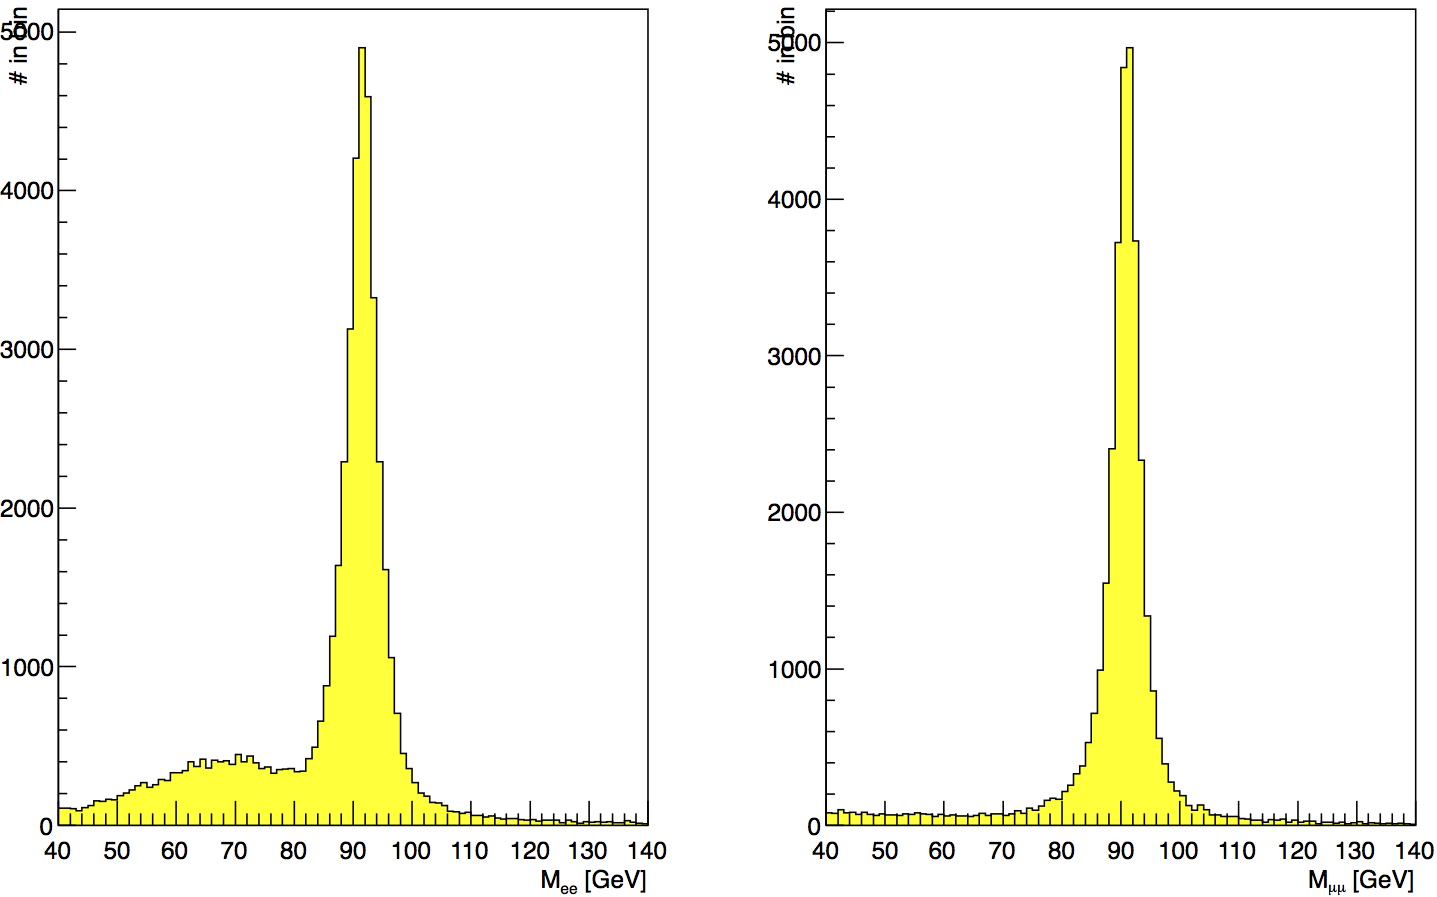
\includegraphics[width=\linewidth]{zpeak2.png}
	\caption{\emph{The invariant mass distribution of 2 electrons (left) and 2 muons (right) originating from the decay of ZZ bosons to 2e2$\mu$. The sharply defined peaks correspond to on-shell Z bosons.
	\\Plot made from ZZ $\rightarrow$ 2e2$\mu$ Monte Carlo}}
	\label{fig:zpeak2}
\end{figure}
\begin{figure}[!h]
	\begin{minipage}[b]{.5\linewidth}
 		\centering
 		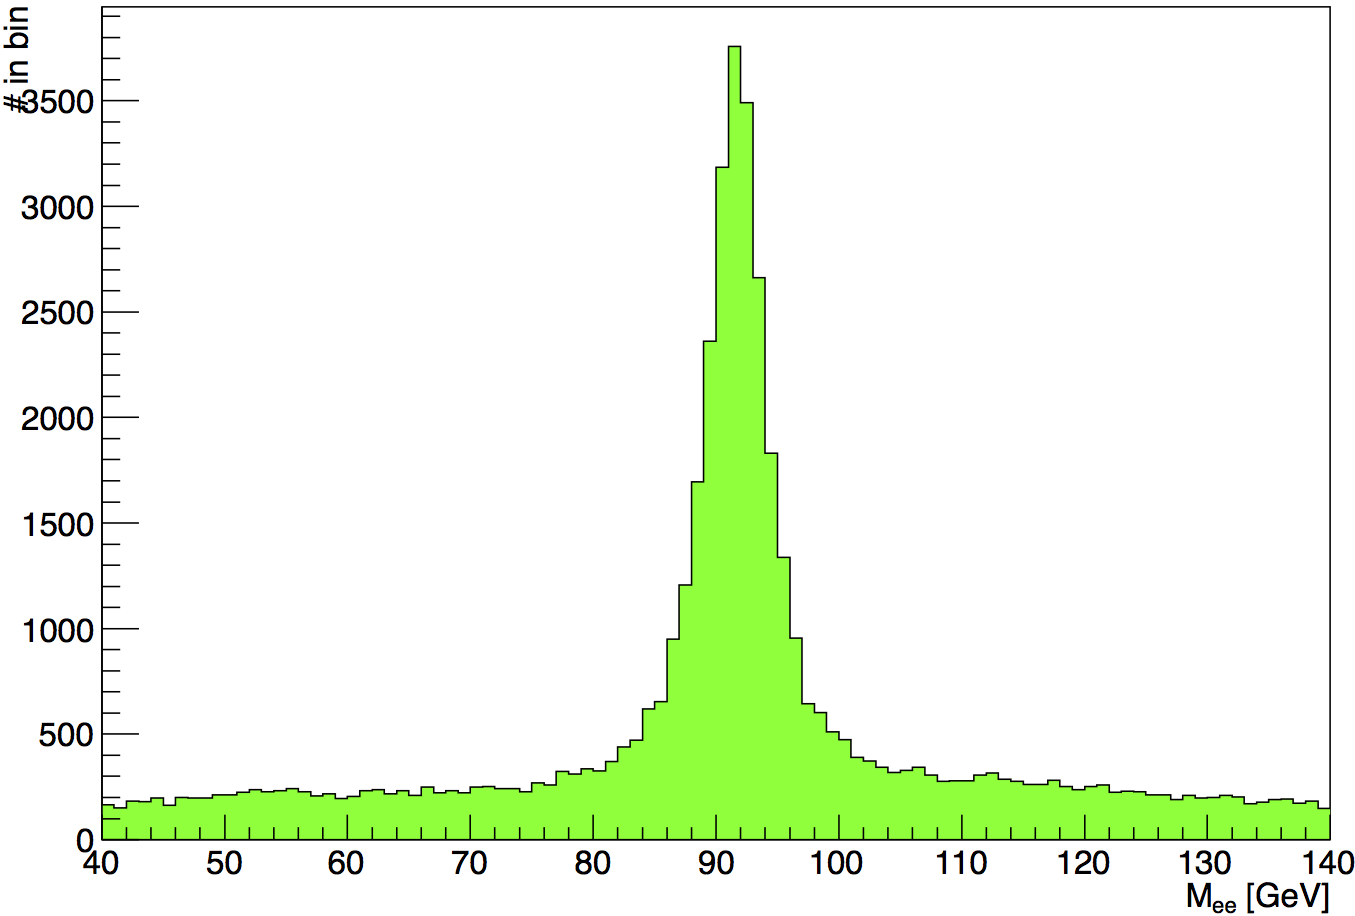
\includegraphics[width=\linewidth]{zpeak1.png}
	\end{minipage}
	\begin{minipage}[b]{.5\linewidth}
 	  	\centering
 	  	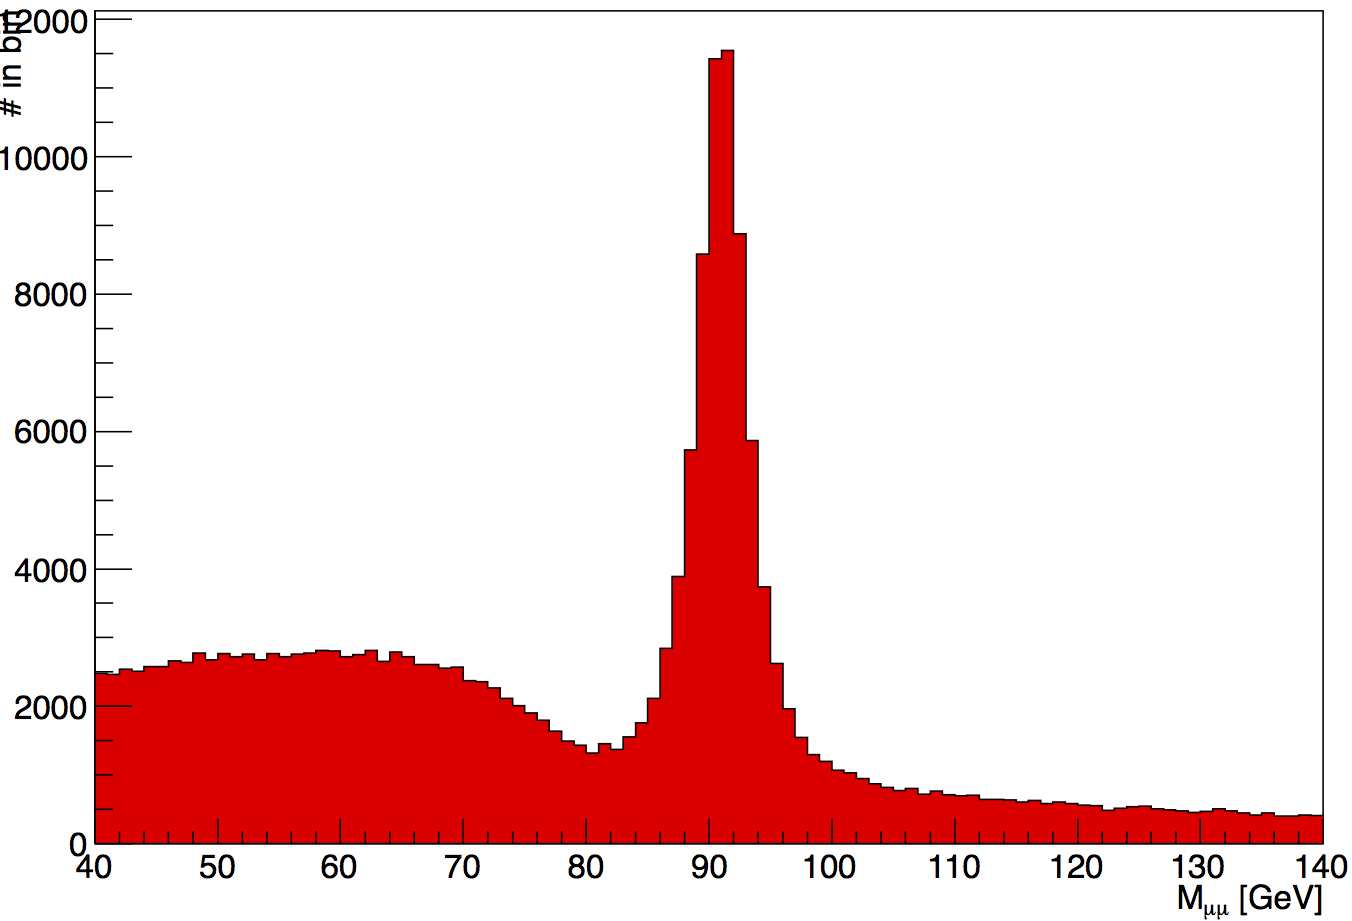
\includegraphics[width=\linewidth]{zpeak3.png}
	\end{minipage}
	\caption{\emph{The invariant mass distribution of 2 electrons (left) and 2 muons (right) originating from the decay of ZZ bosons to 4e (left) or 4$\mu$ (right). The sharply defined peaks correspond to on-shell Z bosons.
	\\Plot made from: 
	\\ZZ $\rightarrow$ 4e Monte carlo (left)
	\\ZZ $\rightarrow$ 4$\mu$ Monte Carlo (right)}}
	\label{fig:zpeak1}
\end{figure}




\subsection{Invariant mass distribution of 4 leptons}
To determine the mass of the Higgs boson, the invariant mass distribution of 4 leptons is established. By comparing the obtained distribution to actual data an excess of event can be noticed. Such an excess of events can be an indication of a new particle such as the Higgs boson.




\subsubsection{Background}
The main background for this analysis is the decay of ZZ boson pairs, of which one Z boson can be off-shell, produced in any process other than Higgs decay. The Monte Carlo simulations used to establish the invariant mass background distribution are listed in table \ref{table:norm1}.




\subsubsection{Event selection}
\begin{floatingtable}[r]{
	\begin{tabular}{l | l}
		\boldmath$\tau^- \rightarrow$			& \textbf{BR (\%)}\\
		\hline
		e$^- \bar\nu_e \nu_\tau$			& 17.85 $\pm$ 0.017\\
		$\mu^- \bar\nu_{\mu} \nu_\tau$		& 17.36 $\pm$ 0.05\\
	\end{tabular}}
	\caption{\emph{Branching ratios for leptonic tau decay \cite{taubr}.}}
	\label{table:taudecay}
\end{floatingtable}
The events relevant to this analysis are those events resulting from the decay of ZZ boson pairs to 4 leptons. The first selection is based on the particles in the final state: only events resulting in exactly (2 electrons and 2 anti- electrons) or (1 electron, 1 anti-electron, 1 muon and 1 anti-muon) or (2 muons and 2 anti-muons) are selected. Though CMS can not detect taus directly, there is a probability that taus produced in the decay of a Z boson decay to muons or electrons. The probability that such a process occurs is dictated directly by the tau branching ratios (table \ref{table:taudecay}). This table allows to calculate the branching ratios for $\tau\tau$ decay. The errors on these branching ratios are computed through error propagation\footnote{
$
\sigma_x = \sqrt{\sum\limits_{i=1}^{n} \left ( \frac{\partial f(x)}{\partial x_i} \cdot \sigma_{xi} \right)}
$
}.
\begin{eqnarray}
	&BR&(\tau\tau\rightarrow\ ee) = BR(\tau\rightarrow\ e) \cdot BR(\tau\rightarrow\ e) = 3.19\pm0.02\%\\
	&BR&(\tau\tau\rightarrow\mu\mu) = BR(\tau\rightarrow\mu) \cdot BR(\tau\rightarrow\mu) = 3.01\pm0.02\%
\end{eqnarray}




\subsubsection{Establishing the 4l mass distribution}
The invariant mass distribution of 4 leptons is governed by the decay of ZZ, ZZ\superscript{*} and Higgs bosons to 4 leptons (and in the case of taus: the decay of taus to muons and/or electrons). Figure \ref{fig:mass1} gives a general idea of the invariant mass distribution in the 4e, 2e2$\mu$ and 4$\mu$ final states.
\begin{figure}[!h]
	\centering
   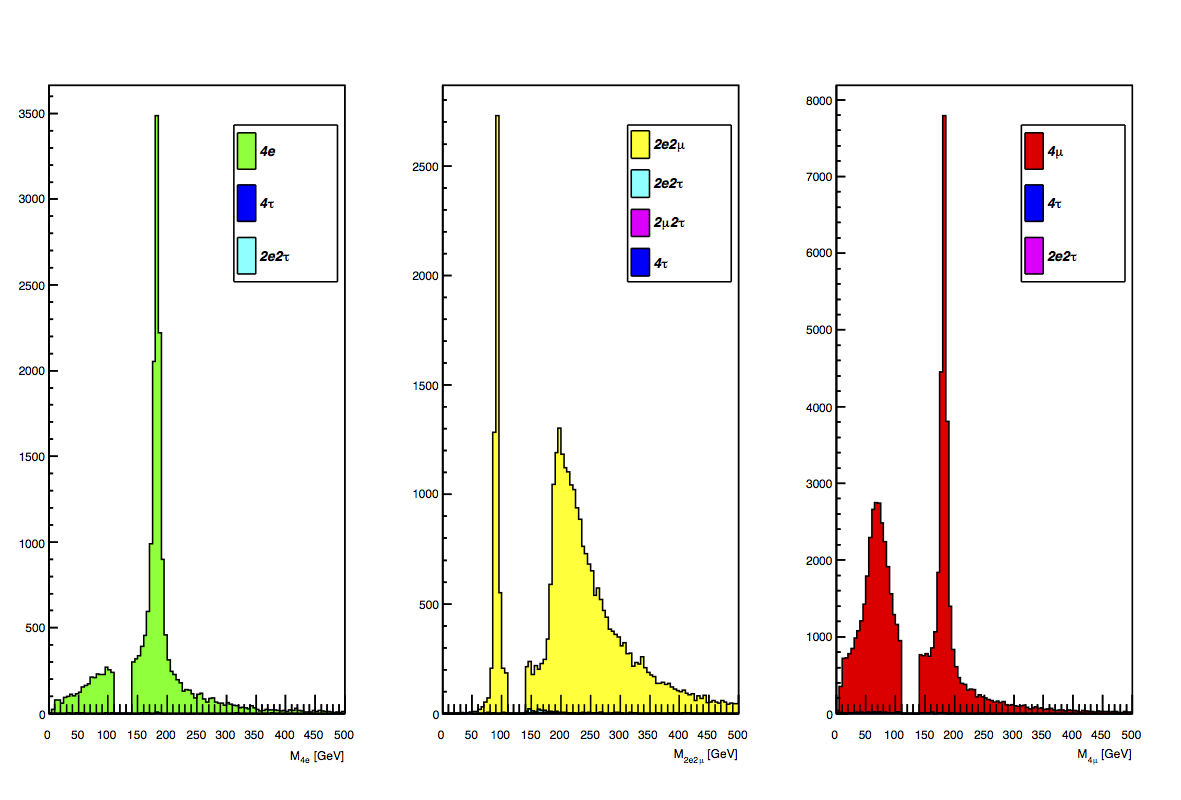
\includegraphics[width=\linewidth]{mass1.png}
   \caption{\emph{The invariant mass distribution over a broad mass spectrum of the 4e respectively 2e2$\mu$ respectively 4$\mu$ final states. The main features of these distributions are the ZZ\superscript{*} peak around 91 GeV, the blinded region around 126 GeV, the on-shell ZZ peak around 182 GeV and the off shell ZZ tail above 182 GeV.
	\\Remark that these distributions are not normalised and no cuts were applied.}
   } \label{fig:mass1}
\end{figure}




\subsubsection{Normalisation}
A significant amount of events is simulated with Monte Carlo simulations. These simulations have to be normalised to match the data. The amount of events (n) of a certain process that occurred in the detector over a certain period of time is dictated by CMS' integrated luminosity ($\mathcal{L}$) and the cross section ($\sigma$) of said process. 
\begin{eqnarray}
	n &=& \sigma \mathcal{L}
\end{eqnarray}
Table \ref{table:norm1} gives an overview of the amount of expected events for the considered processes.
\\By comparing the number of expected events with the number of generated events, it is possible to determine a normalisation factor. This normalisation factor scales the integral of the whole distribution to the required factor. The normalisation factor is
\begin{eqnarray}
	N &=& \frac{\# exp.\ events}{\# gen.\ events}\ =\ \frac{\sigma \mathcal{L}}{\# gen.\ events}
	\label{eq:norm1}
\end{eqnarray}
For the ZZ $\rightarrow$ 2l2l' processes eq. \ref{eq:norm1} is multiplied by a factor 2 because the processes ZZ $\rightarrow$ 2l2l' and ZZ $\rightarrow$ 2l'2l have the same final state in the detector.
\begin{savenotes}
\begin{table}[!hb]
	\centering
	\begin{tabular}{l | l l l | l | l | l}
		\textbf{ZZ}\boldmath$\rightarrow$  
		& \boldmath$\#$ \textbf{Gen.}	
		& \boldmath$\sigma$ \textbf{[fb]}	
		& \boldmath$\mathcal{L}$ \textbf{[fb\superscript{-1}]} 
		& \boldmath$\#$\textbf{exp.}
		& \textbf{Norm.}		
		& \textbf{MC Sample}\\
		
		&\textbf{events}
		&\textbf{@ 8TeV}
		&
		&
		&\textbf{fact}
		&\\
		\hline
		4e							& 1499093	& 76.91				& 19.6		& 1507.4	& 1.006$\times10^{-3}$ 		& ZZTo4e\\
		4$\mu$						& 1499064	& 76.91				& 19.6		& 1507.5	& 1.006$\times10^{-3}$ 		& ZZTo4mu\\
		2e2$\mu$						& 1497445	& 176.7				& 19.6		& 3463.3	& 4.626$\times10^{-3}$		& ZZTo2e2mu\\
		&&&&&\\	
		4$\tau\rightarrow4e$				& 824466		& 7.81$\times10^{-2}$	& 19.6		& 1.53	& 1.856$\times10^{-6}$ 		& ZZTo4tau\\
		4$\tau\rightarrow2e2\mu$			& 824466		& 7.39$\times10^{-2}$	& 19.6		& 1.45	& 8.778$\times10^{-6}$ 		& ZZTo4tau\\
		4$\tau\rightarrow4\mu$			& 824466		& 6.99$\times10^{-2}$	& 19.6		& 1.37	& 1.661$\times10^{-6}$ 		& ZZTo4tau\\
		&&&&&\\	
		2e2$\tau\rightarrow4e$			& 823911		& 5.63				& 19.6		& 110.35	& 2.679$\times10^{-4}$		& ZZTo2e2tau\\
		2e2$\tau\rightarrow2e2\mu$		& 823911		& 5.33				& 19.6		& 104.37	& 2.534$\times10^{-4}$		& ZZTo2e2tau\\

		2$\mu$2$\tau\rightarrow2e2\mu$	& 823922		& 5.63				& 19.6		& 110.35	& 2.679$\times10^{-4}$	 	& ZZTo2mu2tau\\
		2$\mu$2$\tau\rightarrow4\mu$		& 823922		& 5.33				& 19.6		& 104.37	& 2.534$\times10^{-4}$ 		& ZZTo2mu2tau\\

	\end{tabular}
	\caption{\emph{The Monte Carlo simulations used to estimate the background due to ZZ decay with the number of generated events obtained from CMS' Data Aggregation System (DAS), the number of expected events and the normalisation factor.
	\\The cross sections are obtained from literature \cite{analysisnote}. If taus occur as intermediate particles the tau branching ratios are multiplied with the production cross section of the intermediate state. For example: 
	\\$\sigma ( ZZ \rightarrow 2e2\tau \rightarrow 4e ) = \sigma (ZZ \rightarrow 2e2\tau) * BR (\tau \rightarrow e) * BR (\tau \rightarrow e)$}}
	\label{table:norm1}
\end{table}
\end{savenotes}
\\Applying this normalisation rescales the distribution (fig. \ref{fig:mass2}). 
\\The normalised invariant mass distribution is compared to the actual data. There is some discrepancy between Monte Carlo and data in the single Z peak. This is due to the decay of Z bosons to 4 leptons through radiation of a second virtual Z\superscript{*}, for which no simulation samples were available. The normalisation in the ZZ region is not entirely correct. To have the best possible agreement a ratio plot\footnote{A ratio plot is a histogram that compares two other histograms (Monte Carlo and data) by dividing bin by bin. If the histograms are identical, the ratio plot is exactly one.} is established, taking into account the errors in every bin. 
\\The ratio plots (fig. \ref{fig:mass5}) are fitted right of the blinded region, in the ZZ boson peak where the data is expected to match the Monte Carlos. The renormalisation factors obtained from the ratio plots are
\begin{table}[H]
	\centering
	\begin{tabular}{|l l|}
	\hline
	N$'$\subscript{4e}&= 1.19573$\pm$0.458907\\
	N$'$\subscript{2e2$\mu$}&= 1.49419$\pm$0.205079\\
	N$'$\subscript{4$\mu$}&= 1.26262$\pm$0.261496\\
	\hline
	\end{tabular}
\end{table}
The renormalisation factors N$'$\subscript{4e} and N$'$\subscript{4$\mu$} lie (almost) within 1 standard deviation of 1.0 and all three renormalisation factors lie within 1 standard deviation of each other, indicating that the original normalisation is a decent one.
\begin{figure}[!ht]
 	\centering
 	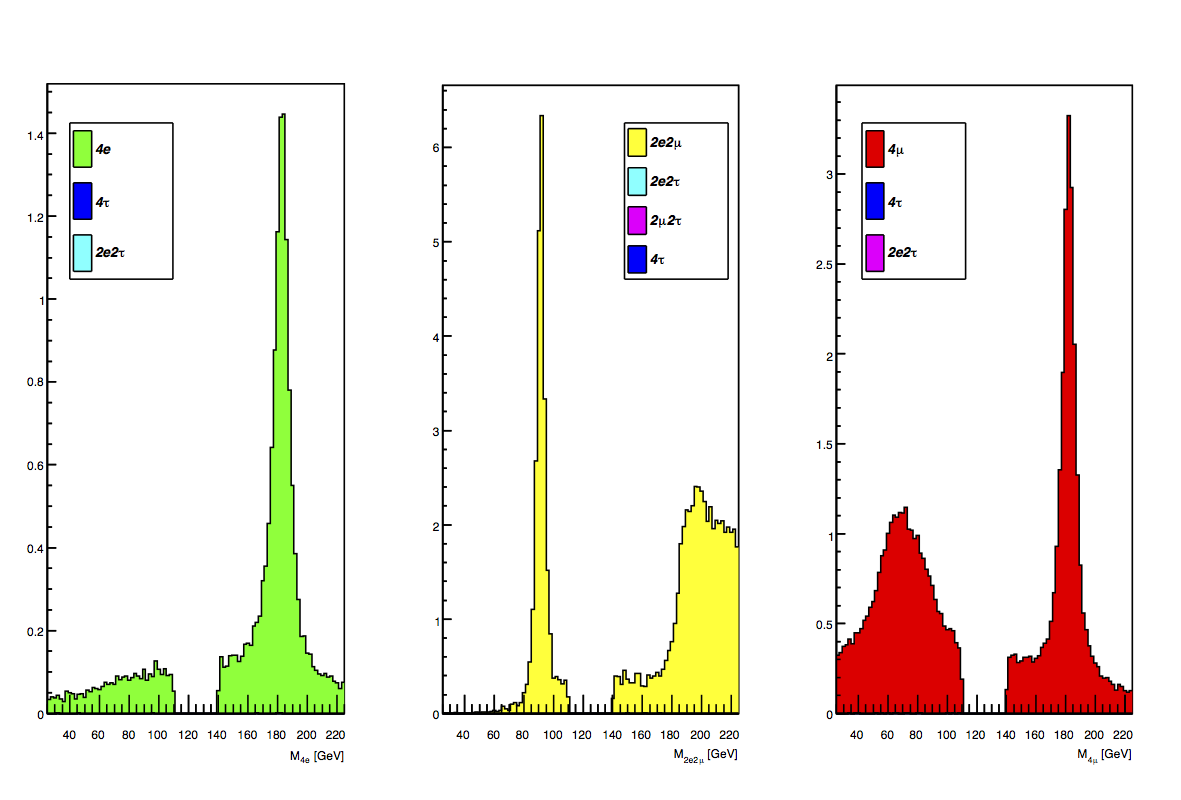
\includegraphics[width=\linewidth]{mass2.png}
	\caption{\emph{The normalised invariant mass distribution over a small focus region of the 4e respectively 2e2$\mu$ respectively 4$\mu$ final states.}}
	\label{fig:mass2}
\end{figure}
\begin{figure}[H]
	\begin{minipage}[b]{.5\linewidth}
 		\centering
 		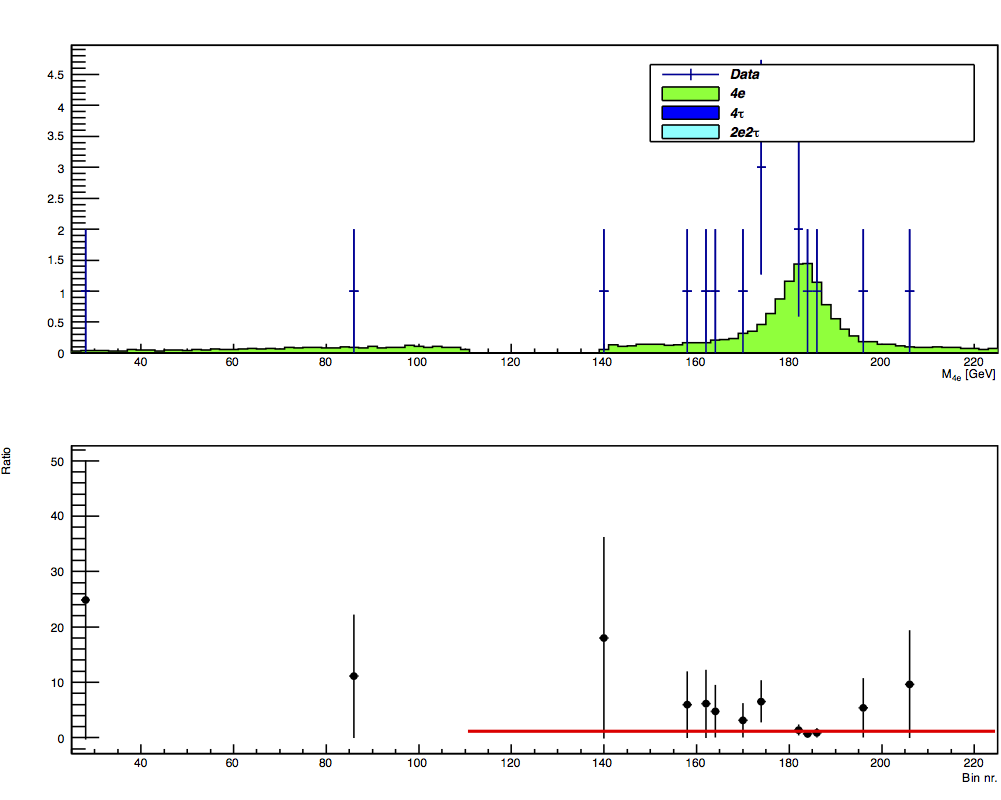
\includegraphics[width=\linewidth]{mass3a.png}
	\end{minipage}
	\begin{minipage}[b]{.5\linewidth}
 	  	\centering
 	  	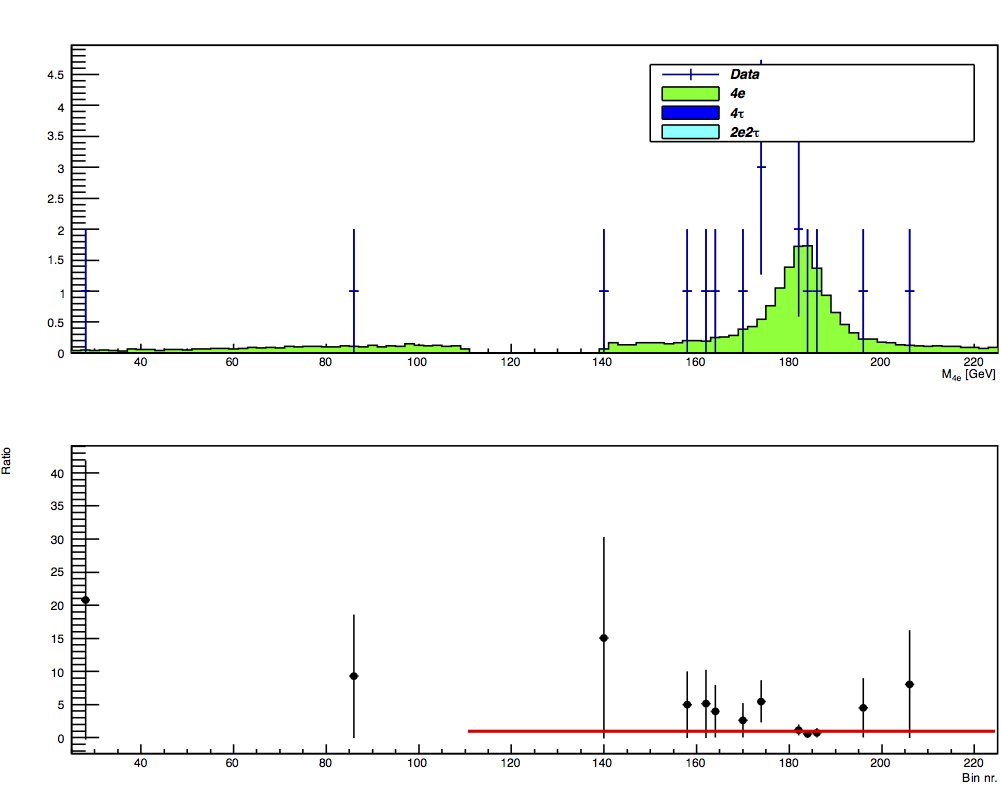
\includegraphics[width=\linewidth]{mass3b.png}
	\end{minipage}
\end{figure}
\begin{figure}[H]
	\begin{minipage}[b]{.5\linewidth}
 		\centering
 		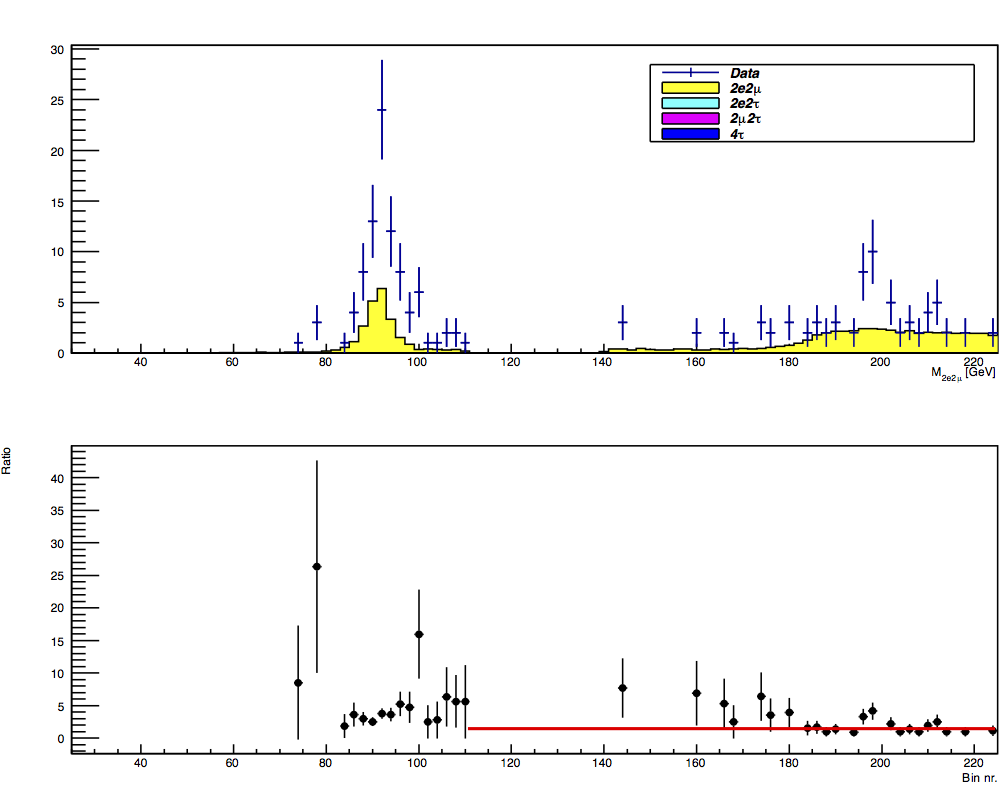
\includegraphics[width=\linewidth]{mass4a.png}
	\end{minipage}
	\begin{minipage}[b]{.5\linewidth}
 	  	\centering
 	  	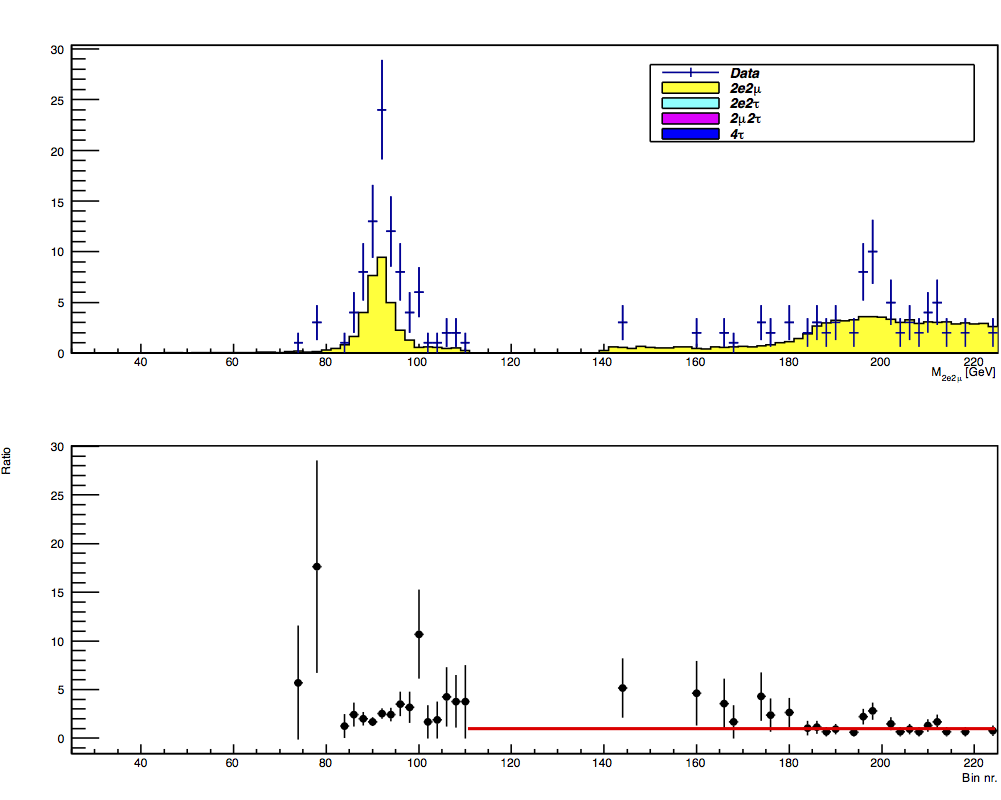
\includegraphics[width=\linewidth]{mass4b.png}
	\end{minipage}
\end{figure}
\begin{figure}[H]
	\begin{minipage}[b]{.5\linewidth}
 		\centering
 		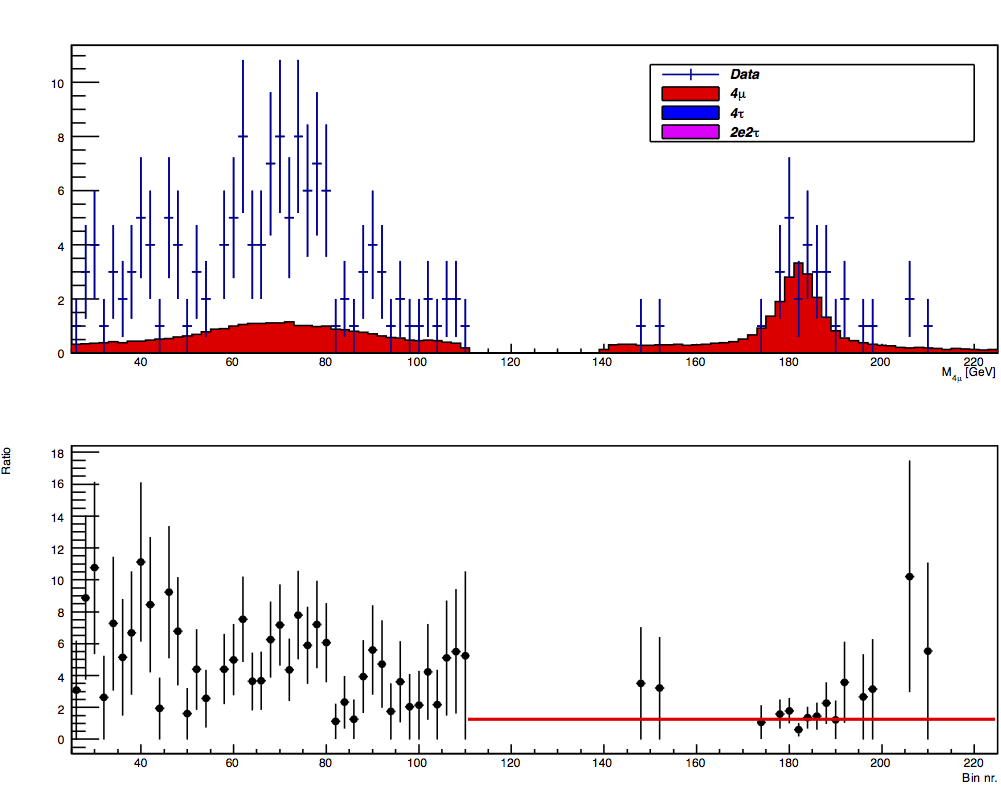
\includegraphics[width=\linewidth]{mass5a.png}
	\end{minipage}
	\begin{minipage}[b]{.5\linewidth}
 	  	\centering
 	  	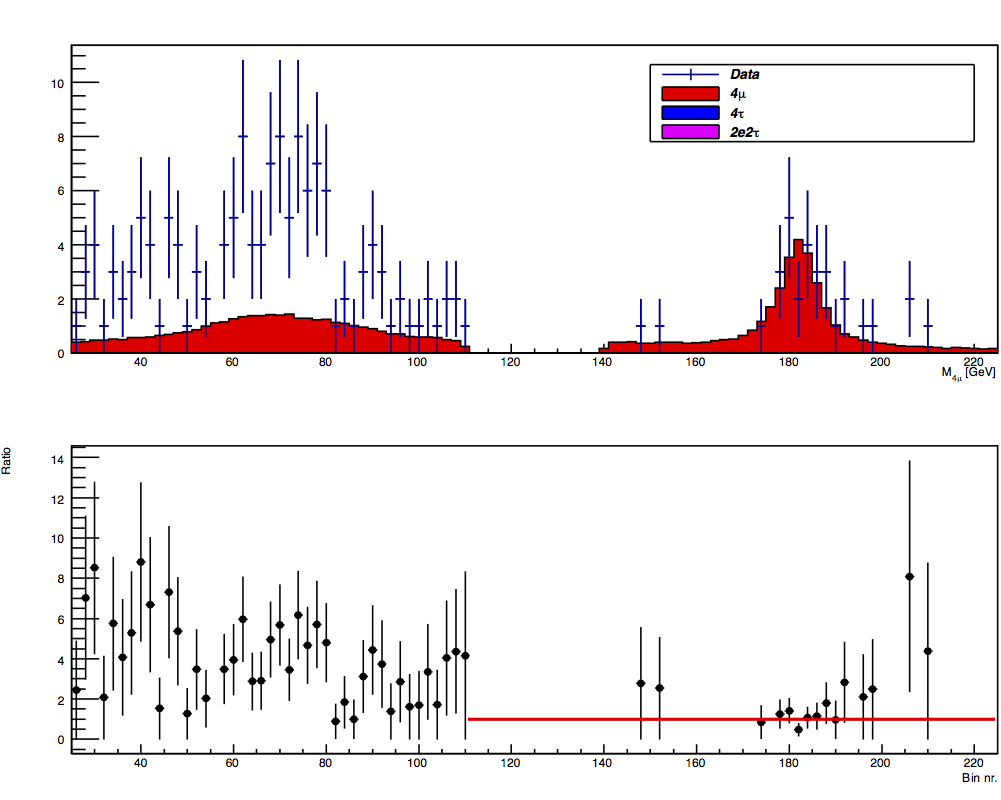
\includegraphics[width=\linewidth]{mass5b.png}
	\end{minipage}
	\caption{\emph{(Left) the invariant mass distribution of 4e respectively 2e2$\mu$ respectively 4$\mu$ before renormalisation. (Right) the same distribution after renormalisation. Remark that the ratio plots run from 110 GeV to 220 Gev. The (empty) blinded region does not contribute to the ratio plots.}}
	\label{fig:mass5}
\end{figure}




\subsubsection{Stacking}
The final distribution includes the 4e, 2e2$\mu$ and 4$\mu$ final states. Once the distributions of the three final states are normalised independently, they can be stacked to establish the total distribution (fig. \ref{fig:mass6}).
\\Remark that the Monte Carlo - data agreement is best in the on-shell ZZ boson peak.
\begin{figure}[!h]
 	\centering
 	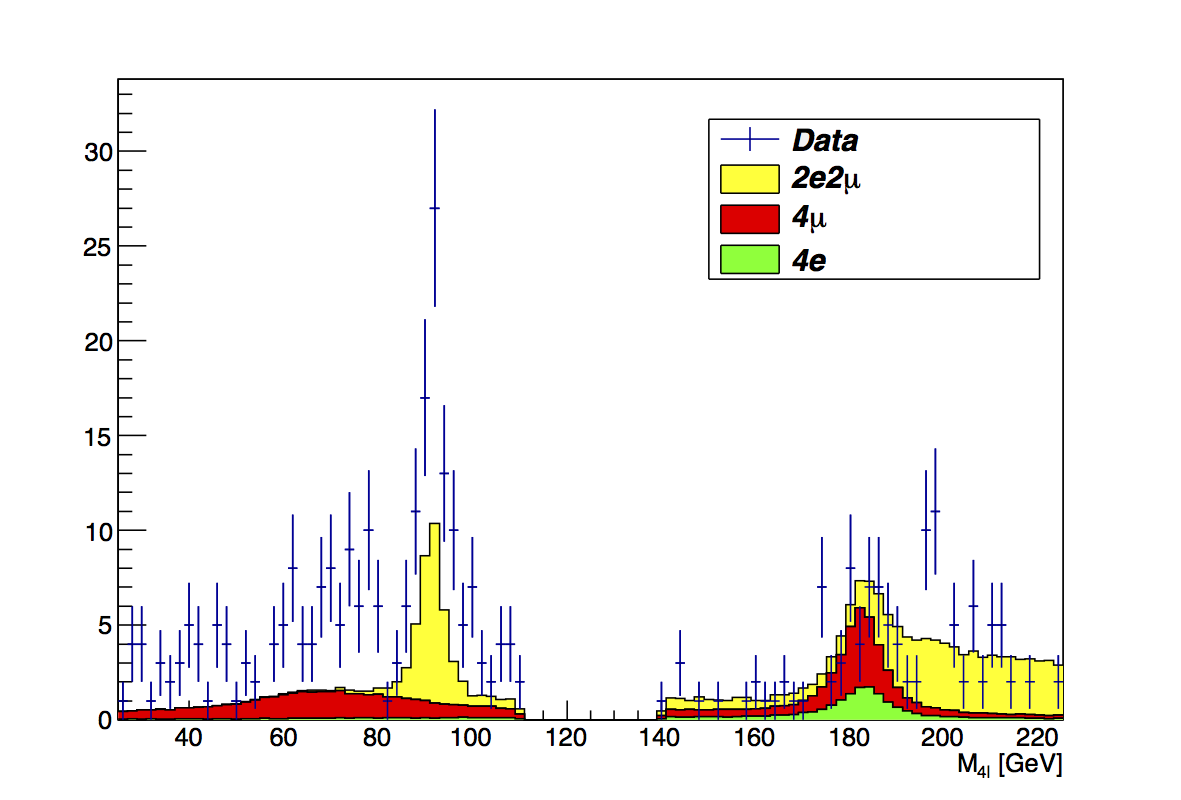
\includegraphics[width=\linewidth]{mass6.png}
	\caption{\emph{The normalised invariant mass distribution of 4 leptons}}
	\label{fig:mass6}
\end{figure}




\subsubsection{Unblinding}
At this stage it is possible to unblind the background distribution. The obtained distribution is the complete normalised background distribution. This distribution only includes the expected background of the H $\rightarrow$ ZZ $\rightarrow$ 4l process. To obtain a usable distribution a signal must be added as well. Monte Carlo simulations for the decay of Higgs bosons are stacked on top of the background. By comparing the obtained distribution with data, conclusions can be drawn. The Monte Carlo signal samples used are listed in table \ref{table:higgs1}.
\begin{table}[H]
	\begin{tabular}{l | l l  | l }
		\textbf{Prod.}  
		& \boldmath$\#$ \textbf{Gen.}	
		& \boldmath$\sigma$ \textbf{[pb]}	
		& \textbf{MC}\\
		
		\textbf{process}
		&\textbf{events}
		&\textbf{@ 8TeV}
		&\textbf{sample}\\
		\hline
		GGF				& 299974		& 18.970		 	& GluGluToHToZZTo4L\_M-126\_8TeV\\
		VBF				& 49945			& 1.5680		 	& VBF\_HToZZTo4L\_M-126\_8TeV\\
	\end{tabular}
	\caption{\emph{The Monte Carlo simulations used to estimate the Higgs signal where a Higgs mass of 126 GeV is assumed. Associated production is not considered in this analysis due to the very small cross section in comparison with gluon gluon fusion and vector boson fusion.
	\\The cross sections were obtained from literature \cite{two}.}}
	\label{table:higgs1}
\end{table}
Before stacking the signal, it has to be normalised. The normalisation factor is defined as
\begin{eqnarray}
	N = \frac{\sigma_{H\ production}\ \mathcal{L}}{\#\ gen.\ ev.}\cdot BR(H\rightarrow ZZ) \cdot BR(Z\rightarrow l^+ l^-) \cdot BR(Z\rightarrow l^{+ '}  \mu^{- '}) \nonumber
	\label{eq:normalisator}
\end{eqnarray}
The production cross sections and number of generated events are listed in table \ref{table:higgs1}. Due to the nature of the signal simulations used (H $\rightarrow$ ZZ) the branching ratio BR(H$\rightarrow$ZZ) in eq. \ref{eq:normalisator} can be set to 1. The branching ratios for leptonic Z boson decay are BR(Z $\rightarrow$ e\superscript{+}e\superscript{-}) = 3.363$\pm$0.004\% and BR(Z $\rightarrow\ \mu$\superscript{+}$\mu$\superscript{-}) = 3.366$\pm$0.007\% \cite{three}.
\newline
The normalisation factors are:
\begin{eqnarray}
	N_{GGF}^{4e} &=& \frac{18.970[pb] \cdot 19.6[fb^{-1}]}{299974}\cdot3.363\cdot10^{-2}\cdot3.3663\cdot10^{-2}\\
	\nonumber\\
	N_{VBF}^{4e} &=& \frac{1.5680[pb] \cdot 19.6[fb^{-1}]}{49945}\cdot3.363\cdot10^{-2}\cdot3.363\cdot10^{-2}\\
	\nonumber\\
	N_{GGF}^{2e2\mu} &=& \frac{18.970[pb] \cdot 19.6[fb^{-1}]}{299974}\cdot3.363\cdot10^{-2}\cdot3.366\cdot10^{-2}\\
	\nonumber\\
	N_{VBF}^{2e2\mu} &=& \frac{1.5680[pb] \cdot 19.6[fb^{-1}]}{49945}\cdot3.363\cdot10^{-2}\cdot3.366\cdot10^{-2}\\
	\nonumber\\
	N_{GGF}^{4\mu} &=& \frac{18.970[pb] \cdot 19.6[fb^{-1}]}{299974}\cdot3.366\cdot10^{-2}\cdot3.366\cdot10^{-2}\\
	\nonumber\\
	N_{VBF}^{4\mu} &=& \frac{1.5680[pb] \cdot 19.6[fb^{-1}]}{49945}\cdot3.366\cdot10^{-2}\cdot3.366\cdot10^{-2}
\end{eqnarray}
\begin{figure}[ht]
	\centering
	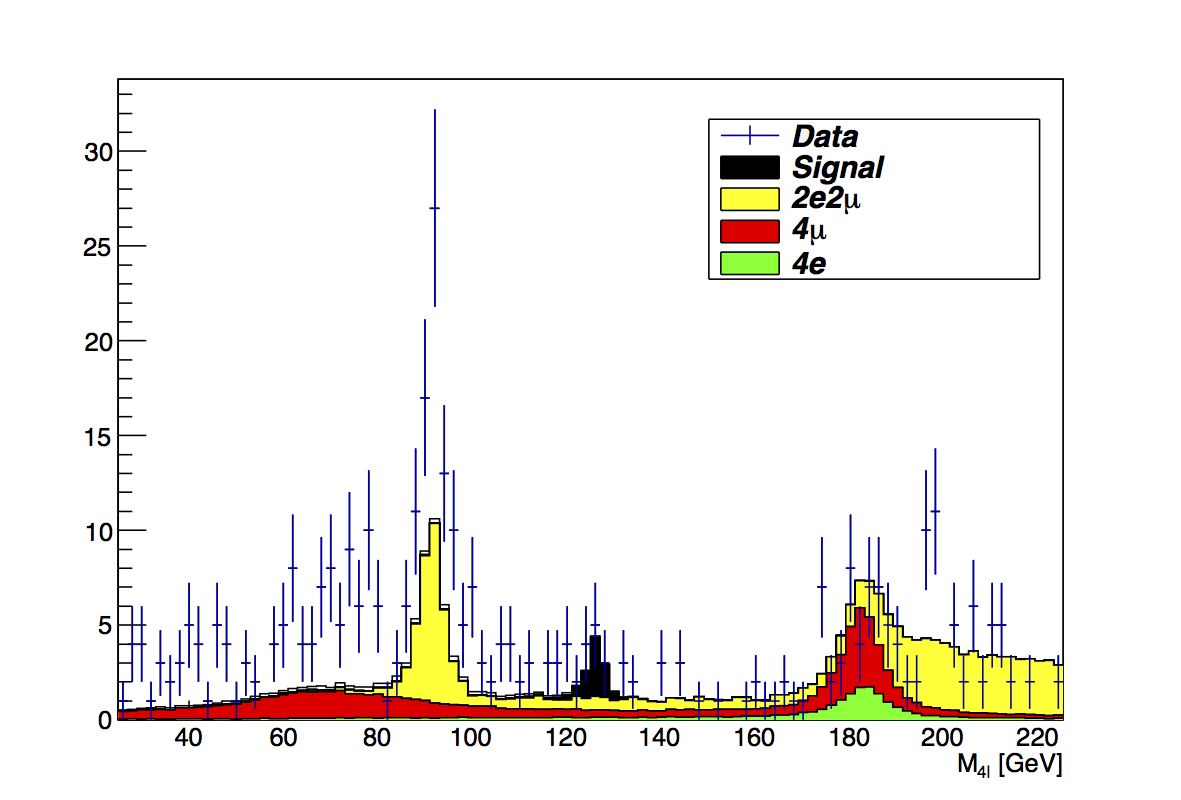
\includegraphics[width=\linewidth]{mass7.png}
	\caption{\emph{The final invariant mass distribution. Completely normalised, with signal and data.}}
	\label{fig:mass7}
\end{figure}

The final step is to unblind the actual data and see how well the expected distribution corresponds to the observed distribution. Figure \ref{fig:mass7} shows the final distribution.
\begin{figure}[H]
	\begin{minipage}[b]{.5\linewidth}
 		\centering
 		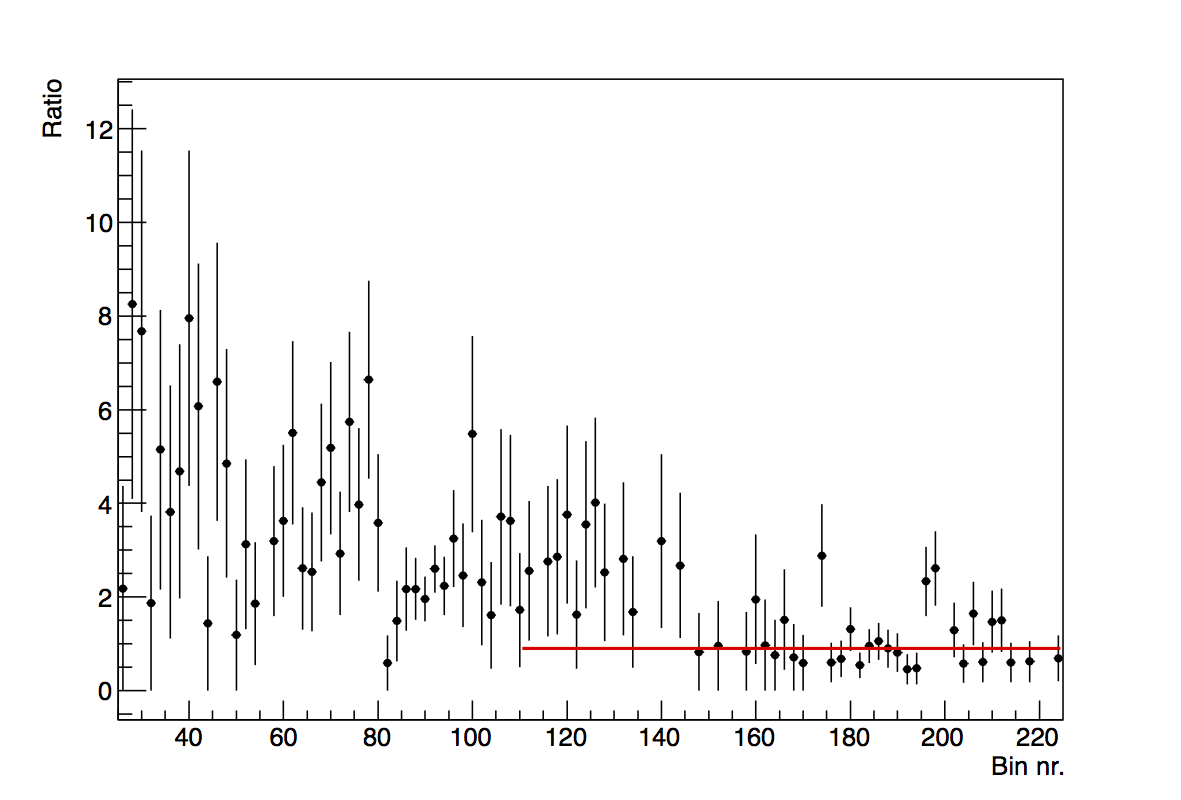
\includegraphics[width=\linewidth]{ratioBackground.png}
	\end{minipage}
	\begin{minipage}[b]{.5\linewidth}
 	  	\centering
 	  	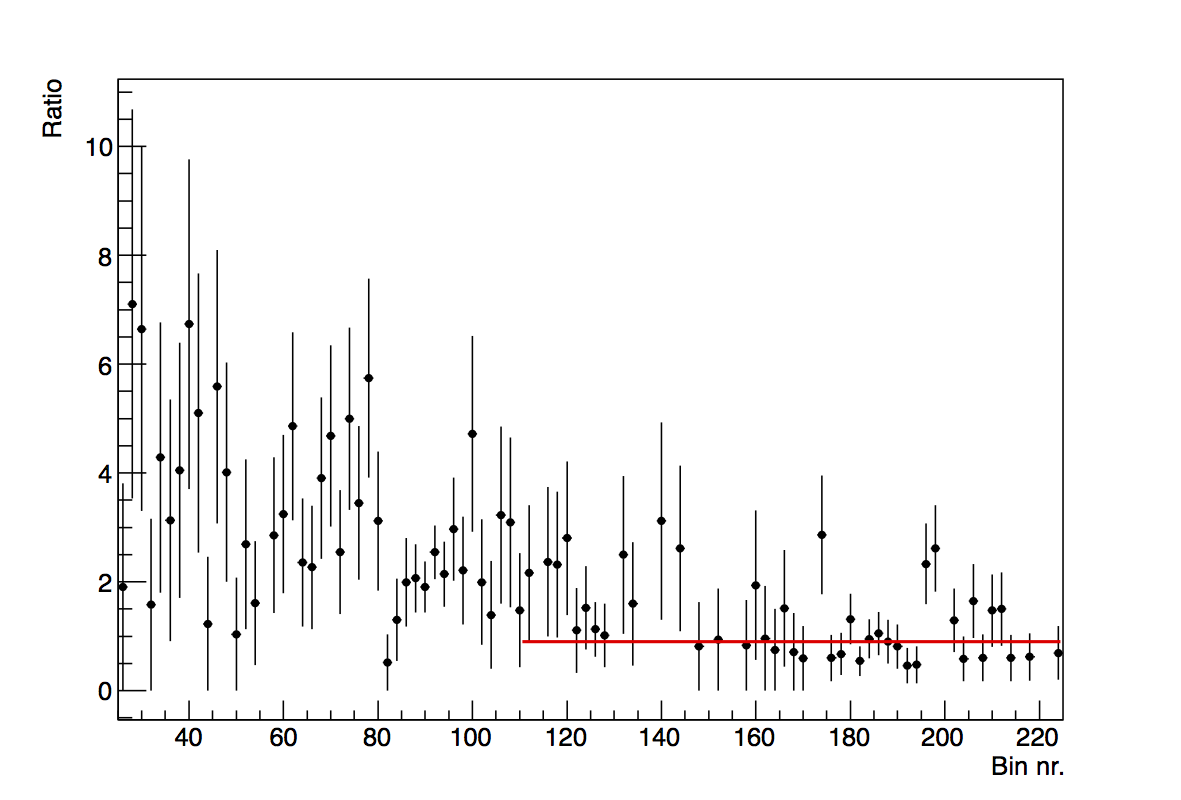
\includegraphics[width=\linewidth]{ratioSignal.png}
	\end{minipage}
	\caption{\emph{(Left) the expected invariant mass distribution of the background divided by the actual data. Remark the discrepancy around 126 GeV. (Right) the invariant mass distribution of the background + signal divided by the actual data. Remark that the ratio is almost 1 around 126 GeV.}}
	\label{fig:ratiofinal}	
\end{figure}
\newpage




\subsection{Statistical analysis}
Data is compared with the expected background + signal distribution (fig. \ref{fig:mass7}). The amount of expected and observed events are summarized in table \ref{table:expected1}. A small excess of events can be seen around 126 GeV.
\\The most important values for significance testing in particle physics are the P value and the z score. Evidence for a new particle is defined by a P score smaller than 0.003 and a z score exceeding 3 standard variations. A discovery can be claimed when the P score is smaller than 0.0000003 and the z score exceeds 5 standard deviations.
\begin{table}
	\centering
	\begin{tabular}{l|lll|l}
		\textbf{Higgs mass}	& \textbf{Background}	& \textbf{Signal} 		& \textbf{Signal +}		& \textbf{Data}\\
							&						& 						& \textbf{background}	&			   \\
		\hline
		121 - 122 [GeV]		&1.23$\pm$0.08		&0.58$\pm$0.03		&1.80$\pm$0.09		&2$\pm$1.41\\
		123 - 124 [GeV]		&1.13$\pm$0.08		&1.50$\pm$0.05		&2.66$\pm$0.09		&4$\pm$2.00\\
		125 - 126 [GeV]		&1.25$\pm$0.08		&3.19$\pm$0.08		&4.44$\pm$0.11		&5$\pm$2.24\\
		127 - 128 [GeV]		&1.19$\pm$0.08		&1.78$\pm$0.06		&2.96$\pm$0.10		&3$\pm$1.73\\
		129 - 130 [GeV]		&1.04$\pm$0.07		&0.48$\pm$0.03		&1.52$\pm$0.08		&0$\pm$0.00\\
	\end{tabular}
		\caption{\emph{The amount of expected background, signal, and background + signal events compared to the amount of observed events.}}
	\label{table:expected1}
\end{table}
\newline
\newline
\textbf{P value \cite{stat}}
\newline
\emph{The P value is the probability that, under the assumption of the null hypothesis, sample variation would yield a result at least as extreme as the observed result.}
\\The null hypothesis (H$_0$): There is no unknown particle capable of decaying in 4 leptons around 126 GeV. The invariant mass distribution of 4 leptons is therefore completely determined by the decay of ZZ and ZZ$^*$ bosons.
\\The alternative hypothesis (H$_1$): There is an unknown particle capable of decaying in 4 leptons around 126 GeV.
\\For every bin the expected P value is given by comparing the background only distribution with the background + signal distribution. The observed P value is given by comparing the background only distribution with the data. If the signal simulation is a good simulation of the physics taking place in CMS, the expected and observed P values should bin for bin yield similar results.
\\Figure \ref{fig:pvalue1} shows that the expected and observed P value is minimal in the 126 GeV bin. The expected P value in the 126 GeV bin is 0.00377255 while the observed P value is 0.000357673. Furthermore figure \ref{fig:pvalue1} shows that the expected and observed P values are similar. This implies that there is some\footnote{Remark that in most other domains a P value smaller than 0.01 would be considered as strong evidence. However, the requirements in particle physics to allow the discovery of a new particle are extremely severe.} evidence against the null hypothesis. 
\newline
\newline
\textbf{Z score}
\newline
\emph{The Z score is the signed number of standard deviations a value lies above the mean.}
\newline
Figure \ref{fig:sigma1} shows the z score for every bin. The expected z score is 2.67178 and the observed z score is 3.38363 in the 126 GeV bin. The z score is maximal in the 126 GeV bin. This is a significant result, but not enough to claim the discovery of a new particle with an invariant mass of about 126 GeV.
\begin{figure}[H]
	\begin{minipage}[b]{.5\linewidth}
 		\centering
 		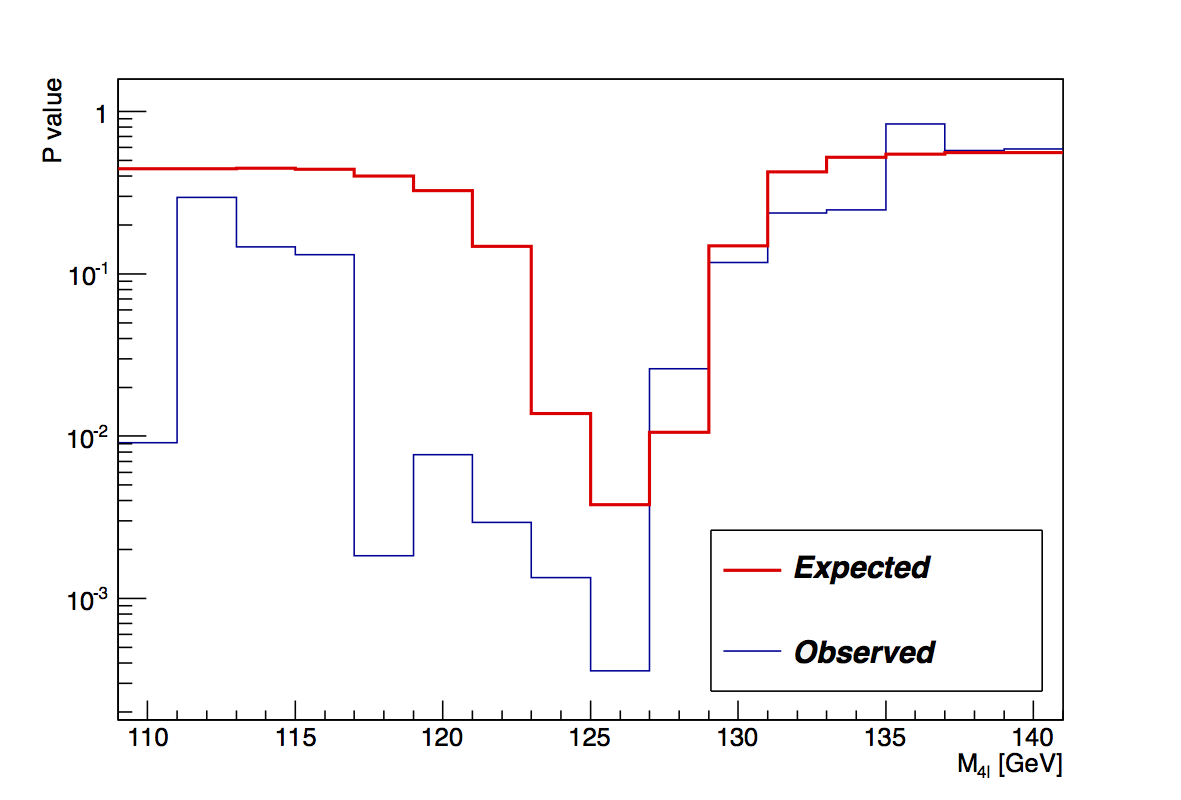
\includegraphics[width=\linewidth]{pvalue.png}
		\caption{\emph{The P value for every bin around 126 GeV. The minimum lies (as expected) in the 126 GeV bin.}}
		\label{fig:pvalue1}
	\end{minipage}
	\begin{minipage}[b]{.5\linewidth}
 	  	\centering
 	  	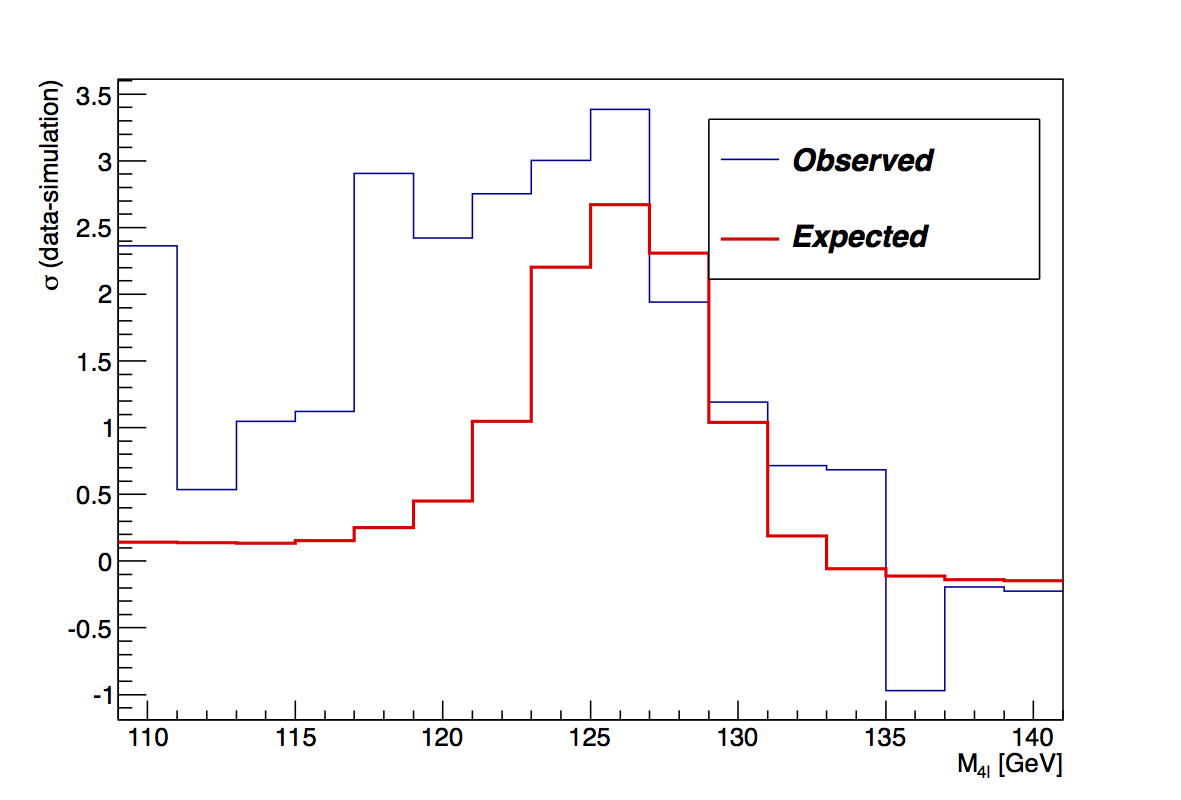
\includegraphics[width=\linewidth]{Sigma.png}
		\caption{\emph{The z score for every bin around 126 GeV. The maximum lies (as expected) in the 126 GeV bin.}}
		\label{fig:sigma1}
	\end{minipage}
\end{figure}




\newpage
\subsection{Proposed cuts}\label{seq:cut} \label{sec:cut1}
The following cuts were proposed but failed to improve the statistical significance of the result while throwing away part of the data. These cuts were tested but not applied.
\\By cutting on certain particle and kinematic properties it is possible to reduce the background while keeping most of the signal.
\newline
\newline
\textbf{P\subscript{T} cut}
\newline
The first discriminating parameter considered is the transverse momentum P\subscript{T} of electrons and muons. Figure \ref{fig:pt1} compares the P\subscript{T} of electrons and muons produced through ZZ decay to the P\subscript{T} of electrons produced through Higgs decay.
\\The distributions of the electrons are rather similar. The electrons' P\subscript{T} distribution has therefore no discriminating power between Monte Carlo and data. The distributions of the muons are more different. A second peak in the ZZ $\rightarrow$ 4l $\rightarrow$ 2e2$\mu$ Monte Carlo simulations P\subscript{T} distribution is not present in the H $\rightarrow$ ZZ $\rightarrow$ 4l $\rightarrow$ 2e2$\mu$ Monte Carlo simulation P\subscript{T} distribution. Cutting away (part of) the second peak cuts a big part of the background while keeping most of the signal.
\begin{figure}[!hb]
	\begin{minipage}[b]{.5\linewidth}
 		\centering
 		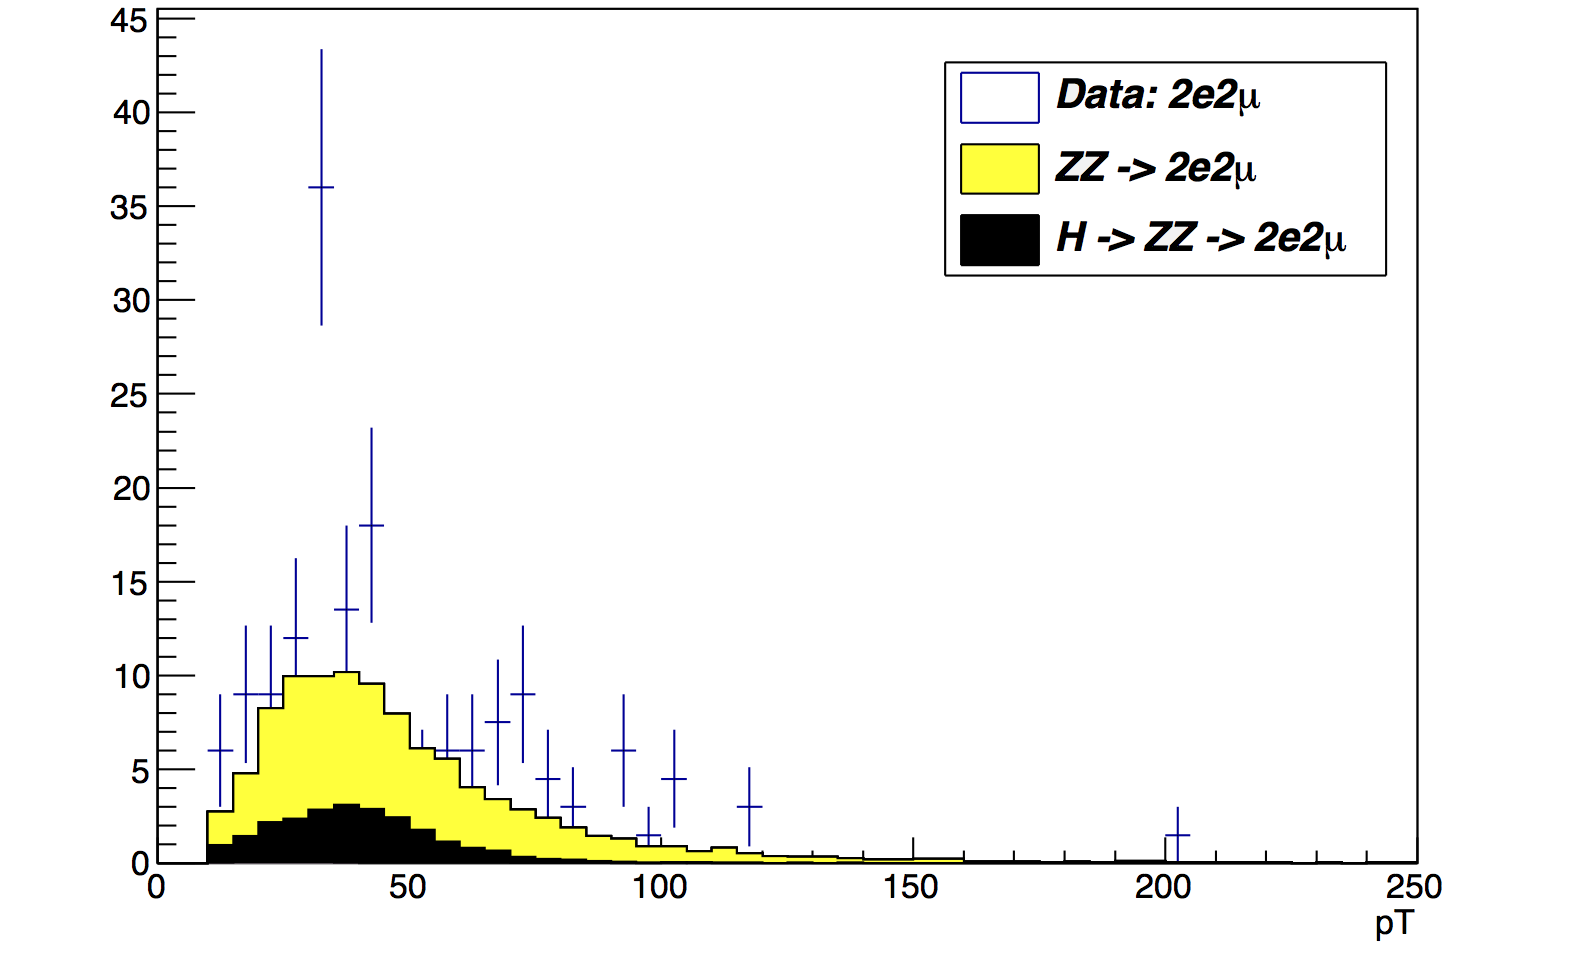
\includegraphics[width=\linewidth]{ptelectrons.png}
	\end{minipage}
	\begin{minipage}[b]{.5\linewidth}
 	  	\centering
 	  	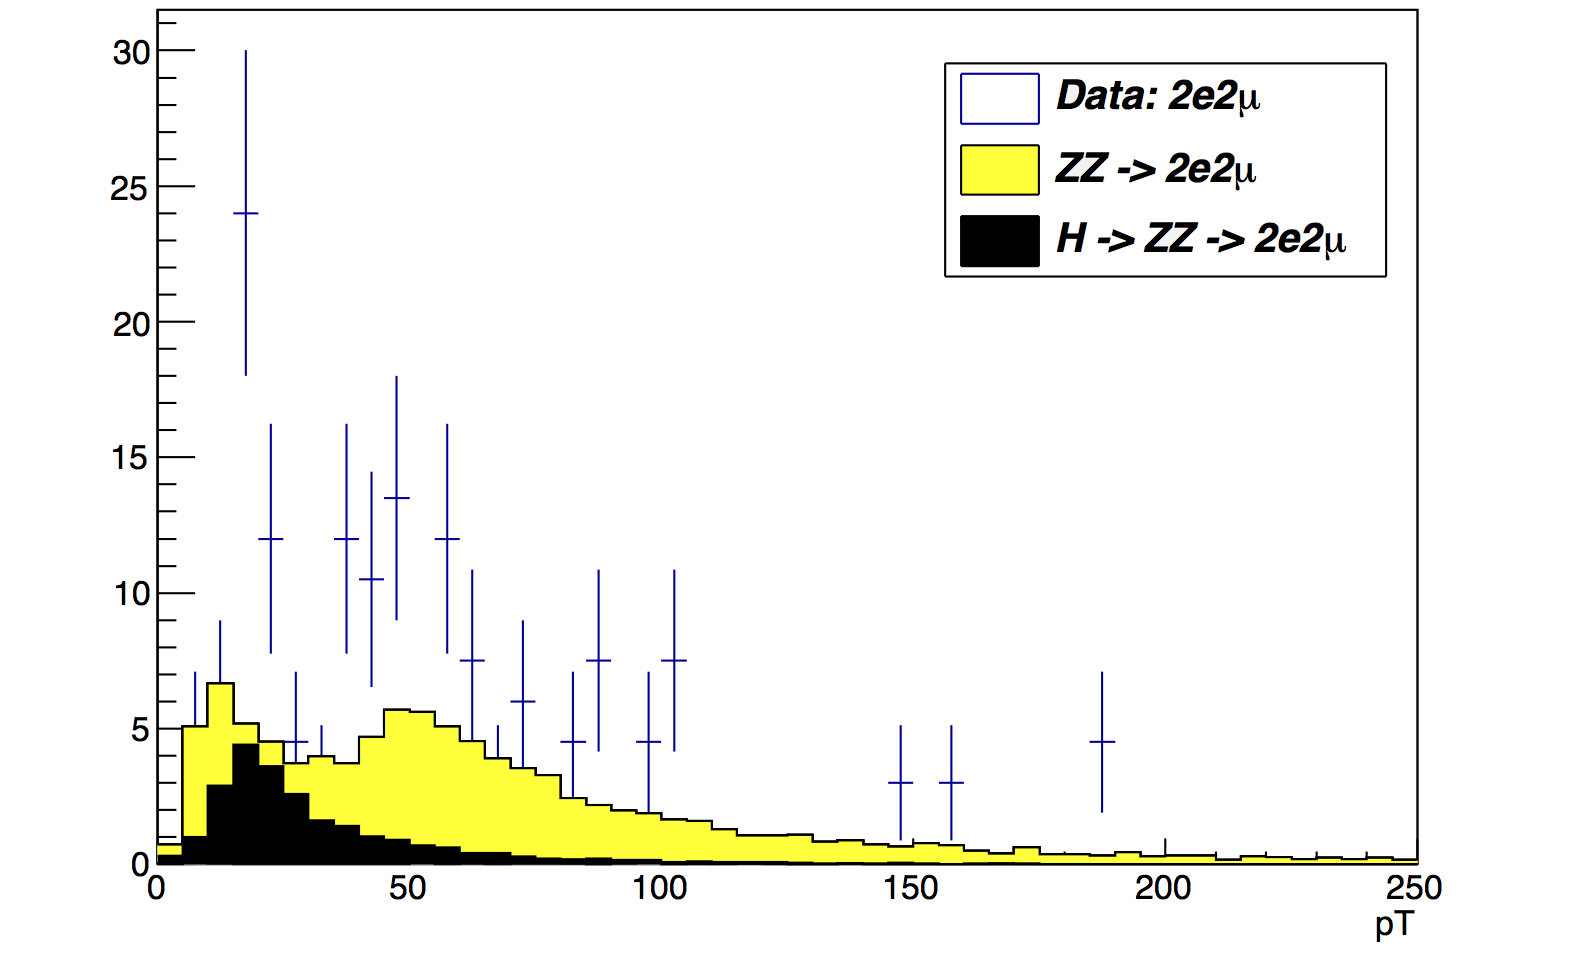
\includegraphics[width=\linewidth]{ptmuons.png}
	\end{minipage}
	\caption{\emph{A comparison between the P\subscript{T} of electrons (left) and muons (right) generated from ZZ decay and H decay. Data represented as well. 
	\\Remark that these histograms are not normalised to the amount of events but to an arbitrary scale factor allowing for the best visual comparison of the distribution shape.}}
	\label{fig:pt1}
\end{figure}
\newline
\textbf{Z\superscript{(*)} mass}
\newline	
The second discriminating parameter considered is the mass of the two separate Z bosons. Figure \ref{fig:zvsz1} shows the mass of the first Z boson as a function of the second Z boson's one. Figure \ref{fig:zvsz1} shows that a cut on the combined mass (80 < M(Z\subscript{1}) + M(Z\subscript{2}) < 130) reduces the background while keeping most of the signal.
\begin{figure}[H]
	\begin{minipage}[b]{0.5\linewidth}
		\centering
		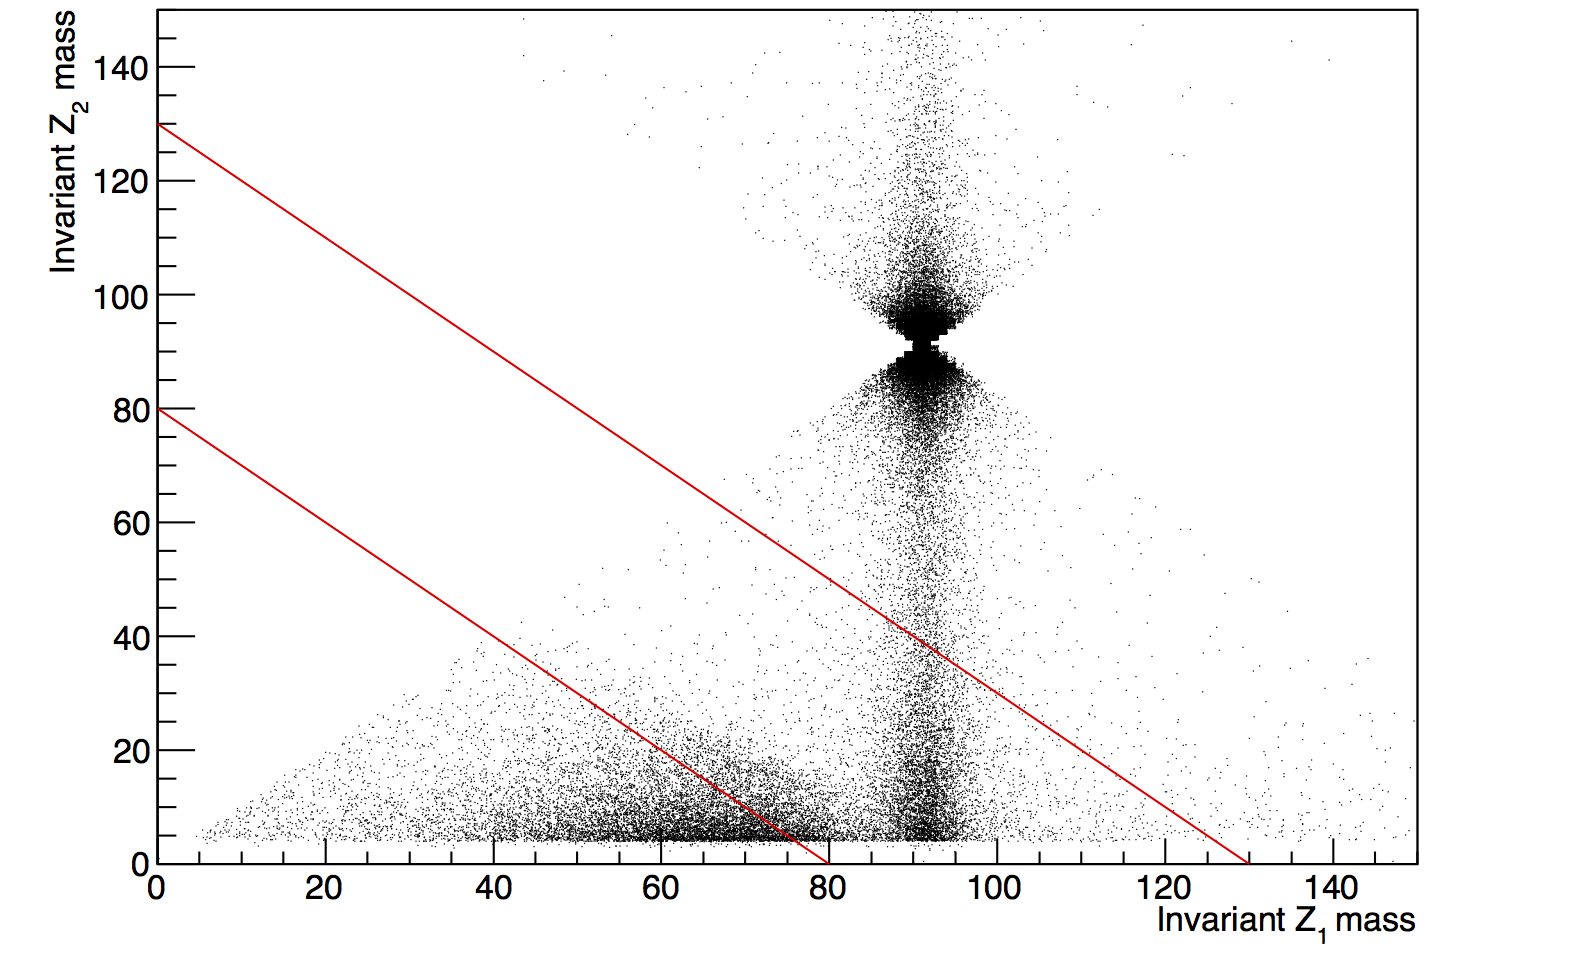
\includegraphics[width=\linewidth]{zvszbackground.png}
	\end{minipage}
	\begin{minipage}[b]{0.5\linewidth}
		\centering
		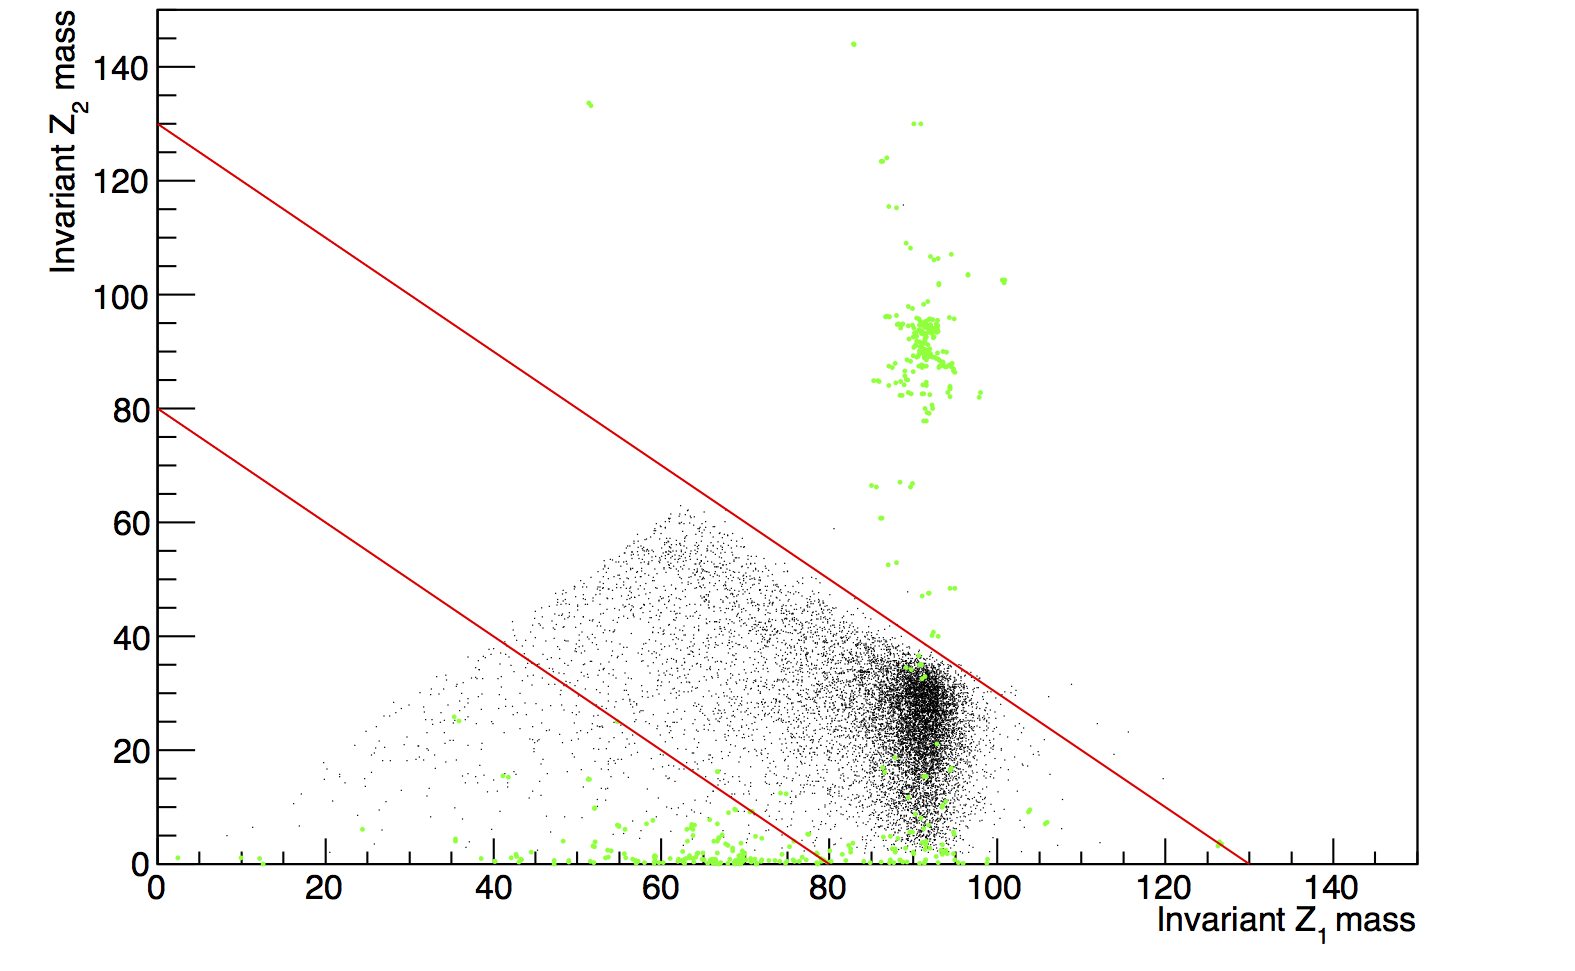
\includegraphics[width=\linewidth]{zvszcombined.png}
	\end{minipage}
	\caption{\emph{Plots of the mass of two Z bosons in function of each other. Cut on the mass: 80 < M(Z\subscript{1}) + M(Z\subscript{2}) < 130.
	\\(Left) Plot made from Monte Carlo simulations of ZZ $\rightarrow$ 4l. The dense central region contains two on-shell Z bosons. The vertical region above Z\subscript{1} = 91 GeV is the region with one on-shell Z boson and one virtual Z boson. One of the criteria for making this plot is that Z\subscript{1}'s mass is closer to 91 GeV than Z\subscript{2}'s mass. This explains the conic shape of the plot.
	\\(Right) Plot made from Monte Carlo simulations of H $\rightarrow$ ZZ $\rightarrow$ 4l. This plot has no events with two on-shell Z bosons. The dense region is dominated by the H $\rightarrow$ ZZ\superscript{*} process. Data is represented in green.}}
	\label{fig:zvsz1}
\end{figure}
\newpage





%----------------------------------------------------------------------------
%Conclusion
%----------------------------------------------------------------------------
\section{Conclusion}
\subsection{Result}
As expected an excess of events was witnessed around 126 GeV with a P value of 0.000357673 and a z score of 3.38363 standard deviations. By convention, this implies there is some evidence for a new particle with a rest mass of 126 GeV, but a more is rigorous analysis needed before claiming a discovery.




\subsection{Error sources}
While the obtained result is statistically significant, it is important to note that there are several sources of errors in this analysis.\\
The main source of errors are the finite resolution of the detector itself, which causes a (small) statistical error on all measurements. Another statistical error occurs when dividing the data in bins.The fit parameters obtained from the ratio plots (p.15) introduce a systematic error. This error on the fitting is the largest of these three errors, but it is the easiest to reduce. This can be done by using all needed Monte Carlo simulations and applying a good normalisation before fitting. 




\subsection{Improving the sensitivity}
The most straight forward way to improve the result is by using not only the $\sqrt s$ = 8 TeV (2012) data but using the $\sqrt s$ = 7 TeV (2010-2011) data as well. Using that data as well does not require any major modifications on the method used in this analysis.
\newline
\newline
The result can be significantly improved by not only considering the H $\rightarrow$ ZZ decay process but also looking at the various decay modes as shown in figure \ref{fig:higgsdecay1}. Including other decay processes does require much more work and the backgrounds for the other processes are more complicated and therefore harder to estimate.
\newline
\newline
Another way of improving the result is by reducing the background by cutting on certain particle and kinematic properties as suggested in \ref{sec:cut1}. The cuts proposed in \ref{sec:cut1} fail to improve the result, therefore smarter cuts have to be chosen to improve the result.
\newpage




%----------------------------------------------------------------------------
%List of figures
%----------------------------------------------------------------------------
\section{List of figures}
\begin{itemize}
	\item figure \ref{fig:sm1}: The Standard Model of Physics. 
	\newline \url{http://en.wikipedia.org/wiki/File:Standard_Model_of_Elementary_Particles.svg}
	
	\item figure \ref{fig:higgsProduction1}: The various production mechanisms for the Higgs boson.
	
	\item figure \ref{fig:higgsdecay1}: The various decay modes of the Higgs boson. 
	\newline \url{https://twiki.cern.ch/twiki/bin/view/LHCPhysics/CrossSections}
	
	\item figure \ref{fig:cms1}: The CMS detector and its main components.
	\newline \url{http://cms.web.cern.ch/news/cms-detector-design}
		
	\item figure \ref{fig:etacms1}: The pseudorapidity at CMS.
	\newline \url{http://www.hephy.at/user/friedl/diss/html/node8.html}
		
	\item figure \ref{fig:eta1}: The pseudorapidity for leptons at CMS.

	\item figure \ref{fig:zpeak2}, \ref{fig:zpeak1}: The mass of a Z boson.
	
	\item figure \ref{fig:mass1}: The 4e, 2e2$\mu$ and 4$\mu$ background before normalisation.
	
	\item figure \ref{fig:mass2}: The 4e, 2e2$\mu$ and 4$\mu$ background normalised to theory.

	\item figure \ref{fig:mass5}: The 4e, 2e2$\mu$ and 4$\mu$ ratio plots used to obtain the best data - Monte Carlo agreement.

	\item figure \ref{fig:mass6}: The normalised invariant mass distribution of 4 leptons.

	\item figure \ref{fig:mass7}: The normalised invariant mass distribution of 4 leptons with data, signal and ratio plot.
	
	\item figure \ref{fig:ratiofinal}: The final ratio plots.
	
	\item figure \ref{fig:pvalue1}: The expected and observed p values for various Higgs masses.
	
	\item figure \ref{fig:sigma1}: The expected and observed z score for various Higgs masses.
	
	\item figure \ref{fig:pt1}: The P\subscript{T} for leptons at CMS.
	
	\item figure \ref{fig:zvsz1}: The mass of two Z bosons in function of each other.
	
\end{itemize}
	
	
	
	
%----------------------------------------------------------------------------
%Bibliografie
%----------------------------------------------------------------------------
\clearpage
\addcontentsline{toc}{section}{\textbf{References}}
\begin{thebibliography}{99}
	\bibitem{sm} A. Romanino, \emph{The Standard Model of Particle Physics}, SISSA/ISAS and INFN.
	\\ \url{http://www.slac.stanford.edu/econf/C0907232/pdf/001.pdf}
	
	\bibitem{paper1} F. Englert, R. Brout, \emph{Broken symmetry and the mass of gauge vector mesons}, Phys. Rev. Letters 13 (1964) 321. 
	\\ \url{http://journals.aps.org/prl/pdf/10.1103/PhysRevLett.13.321}
	
	\bibitem{paper2} P. W. Higgs, \emph{Broken symmetries and the masses of gauge bosons}, Phys. Rev. Letters 13 (1964) 508.
	\\ \url{http://journals.aps.org/prl/pdf/10.1103/PhysRevLett.13.508}
	
	\bibitem{paper3} G. S. Guralnik, C. R. Hagen, T. W. B. Kibble, \emph{Global conservation laws and massless particles}, Phys. Rev. Letters 13 (1964) 585.
	\\ \url{http://journals.aps.org/prl/pdf/10.1103/PhysRevLett.13.585} 
	
	\bibitem{two} LHC Higgs Cross Section Working Group, S. Heinemeier, C. Mariotti, G. Passarino, R. Tanaka (Eds.), \emph{Handbook of LHC Higgs Cross Sections: 3. Higgs Properties}, CERN–2013–004 (CERN, Geneva, 2013), DOI: 10.5170/CERN–2013–004
	\\ \url{http://arxiv.org/pdf/1307.1347v2.pdf}
		 
	\bibitem{branching} A. Denner, S. Heinemeyer, I. Puljak, D. Rebuzzi, M. Spira, \emph{Standard Model Higgs-Boson Branching Ratios with Uncertainties}, arXiv:1107.5909v2 [hep-ph]
	\\ \url{http://arxiv.org/pdf/1107.5909v2.pdf}
	
	\bibitem{cern} The CMS Collaboration, \emph{A New Boson with a Mass of 125 GeV Observed with the CMS Experiment at the Large Hadron Collider}, Science 338, 1569 (2012).
	\\ \url{http://www.sciencemag.org/content/339/6125/1275.2.full.html}
	
	\bibitem{one} The CMS Collaboration, \emph{Analysis note: Properties of the Higgs-like boson in the decay H $\rightarrow$ ZZ $\rightarrow$ 4l in pp collisions at sqrt(s)=7 and 8 TeV}, 04 January 2013, available on CMS information server.

	\bibitem{cms} C-E. Wulz, \emph{The CMS experiment at CERN}, The CMS Collaboration.
	\\ \url{http://www.hephy.at/fileadmin/user_upload/Publikationen/SPIE-5948-21.pdf}

	\bibitem{relativity} D. J. Griffiths, \emph{Introduction to electrodynamics and special relativity}, Reed College, 3rd edition.
		
	\bibitem{taubr} 	K.G. Hayes, \emph{$\tau$ branching fractions}, Hillsdale College, april 2010.
	\url{http://pdg.lbl.gov/2010/reviews/rpp2010-rev-tau-branching-fractions.pdf}
		
	\bibitem{analysisnote} The HZZ4l team (CERN), \emph{Search for the standard model Higgs boson in the decay channel H to ZZ to 4l in pp collisions}, 04 January 2013 (v6, 13 February 2013)

	 \bibitem{three}J. Beringer et al. (Particle Data Group), \emph{Z Mass}, PR D86, 010001 (2012)  \\ \url{http://pdg.lbl.gov})
	 
	 \bibitem{stat}P. K. Sinervo, \emph{Signal Significance in Particle Physics}, hep-ex/0208005 \\
	 \url{http://arxiv.org/abs/hep-ex/0208005v1}

\end{thebibliography} 




\end{document}
%----------------------------------------------------------------------------
%End document
%----------------------------------------------------------------------------
